\documentclass{article}
% \IEEEoverridecommandlockouts
% The preceding line is only needed to identify funding in the first footnote. If that is unneeded, please comment it out.
\usepackage{cite}
\usepackage{amsmath,amssymb,amsfonts}
\usepackage{graphicx}
\usepackage{textcomp}
\usepackage{float}
\usepackage{xcolor}
\usepackage{tikz}
\usepackage{mdframed}
\usepackage{hyperref}
\usepackage{algorithm}
\usepackage{caption}
\usepackage{algpseudocode}
\usepackage{accents}
\usepackage{pgfplots}
\usepackage{filecontents}  
\usepackage{listings}

\usetikzlibrary{matrix}

\newcommand{\gridCellWidth}{0.3}
\newcommand{\gridSize}{7}
\newcommand{\gridSpacing}{0.9}
\newcommand{\gridWidth}{\gridSize*\gridCellWidth}

\newcommand{\gridAxisHorizontalCellColour}{myGreen}
\newcommand{\gridAxisVerticalCellColour}{myOrange}
\newcommand{\gridAxisMiddleColour}{myYellow}
\newcommand{\gridTwoStart}{\gridWidth + \gridSpacing}
\newcommand{\gridThreeStart}{2*\gridWidth + 2*\gridSpacing}

\newcommand{\graphLineSpacing}{0.5}
\newcommand{\graphTensorSpacing}{1}
\newcommand{\graphTensorTwoStart}{1.5*\graphTensorSpacing}
\newcommand{\graphTensorThreeStart}{\graphTensorTwoStart+ 2*\graphTensorSpacing}
\newcommand{\graphTensorFourStart}{\graphTensorThreeStart+ 2*\graphTensorSpacing}

% \def\BibTeX{{\rm B\kern-.05em{\sc i\kern-.025em b}\kern-.08em
%     T\kern-.1667em\lower.7ex\hbox{E}\kern-.125emX}}
\begin{document}

\definecolor{myGreen}{RGB}{95,173,86}
\definecolor{myYellow}{RGB}{242,193,78}
\definecolor{myOrange}{RGB}{247,129,84}
\definecolor{myBlue}{RGB}{118,146,255}
\definecolor{myBrown}{RGB}{90,42,39}
\definecolor{myGrey}{RGB}{238, 228, 225}
\definecolor{myFigureColour}{RGB}{240, 240, 240}

\title{TensorStencil Report}

% \author{\IEEEauthorblockN{Robert Buxton}
% \IEEEauthorblockA{rb419@ic.ac.uk}}

\maketitle

% \begin{abstract}

% \end{abstract}

% \begin{IEEEkeywords}
% Todo
% \end{IEEEkeywords}


\section{Abstract}
We propose an alternative to the ADD METHODS method for stencil computation.
Using tensors contractions use to represent stencil time step updates we can calculate the state of input data after an arbitrary number of time steps in a single pass.
The algorithm can make better use of recent TPU/GPU developments as it is primarily time bound by two groups of matrix multiplications.
\\ \\ This leads to an algorithm that is a for an $k$ dimensional stencil computing $t$ timesteps $O(n^{k+1})$ as opposed to classical loop algorithms which are $O(n^{k}t)$.

\section{Background}


\section{Introduction}
% Todo (Make better use of tensor cores/gpu matrix multipliers for stencil computation)
% \section{Method}
% I propose an alternative to the classical iterative loop method for stencil computation. 
% Using the emergent properties of the transformation matrices use to represent stencil time step update we can calculate the state of input data after an arbitrary number of time steps. 

\subsection{Representing a stencil as matrix multiplications}

The first step we need to take is to represent the star stencil loop in terms of a matrices multiplications.
This isn't very difficult as any star stencil can just be broken down into a individual transformation matrix for each of it's dimensions \cite{10.1145/3524059.3532392}.
The example below is for a 2D 5 wide star stencil. \\

\begin{figure}[H]
	\begin{mdframed}[backgroundcolor=myFigureColour]
		\newcommand{\gridCellWidth}{0.3}
\newcommand{\gridSize}{7}
\newcommand{\gridSpacing}{0.9}
\newcommand{\gridWidth}{\gridSize*\gridCellWidth}
\definecolor{myGreen}{RGB}{95,173,86}
\definecolor{myYellow}{RGB}{242,193,78}
\definecolor{myOrange}{RGB}{247,129,84}
\newcommand{\gridAxisHorizontalCellColour}{myGreen}
\newcommand{\gridAxisVerticalCellColour}{myOrange}
\newcommand{\gridAxisMiddleColour}{myYellow}
\newcommand{\gridTwoStart}{\gridWidth + \gridSpacing}
\newcommand{\gridThreeStart}{2*\gridWidth + 2*\gridSpacing}

\begin{tikzpicture}[every node/.style={minimum size=\gridCellWidth cm-\pgflinewidth, outer sep=0pt}]

%Grid 1

\draw[step=\gridCellWidth cm,color=black] (0,0) grid (\gridWidth,\gridWidth);

\node[fill={\gridAxisHorizontalCellColour}] at (1.5*\gridCellWidth,3.5*\gridCellWidth){};
\node[fill={\gridAxisHorizontalCellColour}] at (2.5*\gridCellWidth,3.5*\gridCellWidth){};
\node[fill={\gridAxisHorizontalCellColour}] at (4.5*\gridCellWidth,3.5*\gridCellWidth){};
\node[fill={\gridAxisHorizontalCellColour}] at (5.5*\gridCellWidth,3.5*\gridCellWidth){};


\node at (1.5*\gridCellWidth,3.5*\gridCellWidth) {\footnotesize x1};
\node at (2.5*\gridCellWidth,3.5*\gridCellWidth) {\footnotesize x2};
\node at (4.5*\gridCellWidth,3.5*\gridCellWidth) {\footnotesize x3};
\node at (5.5*\gridCellWidth,3.5*\gridCellWidth) {\footnotesize x4};


\node[fill={\gridAxisVerticalCellColour}] at (3.5*\gridCellWidth,1.5*\gridCellWidth){};
\node[fill={\gridAxisVerticalCellColour}] at (3.5*\gridCellWidth,2.5*\gridCellWidth){};
\node[fill={\gridAxisVerticalCellColour}] at (3.5*\gridCellWidth,4.5*\gridCellWidth){};
\node[fill={\gridAxisVerticalCellColour}] at (3.5*\gridCellWidth,5.5*\gridCellWidth){};

\node at (3.5*\gridCellWidth,1.5*\gridCellWidth) {\footnotesize y4};
\node at (3.5*\gridCellWidth,2.5*\gridCellWidth) {\footnotesize y3};
\node at (3.5*\gridCellWidth,4.5*\gridCellWidth) {\footnotesize y2};
\node at (3.5*\gridCellWidth,5.5*\gridCellWidth) {\footnotesize y1};


\node[fill={\gridAxisMiddleColour}] at (3.5*\gridCellWidth,3.5*\gridCellWidth){};

\node at (3.5*\gridCellWidth,3.5*\gridCellWidth) {\footnotesize m};

\node[fill={\gridAxisMiddleColour}] at (\gridTwoStart + 3.5*\gridCellWidth,3.5*\gridCellWidth){};
\node at (\gridTwoStart + 3.5*\gridCellWidth,3.5*\gridCellWidth) {\tiny{$\frac{\text{m}}{2}$} };

%Grid 2

\draw[step=\gridCellWidth cm,color=black] (\gridThreeStart,0) grid (\gridWidth + \gridThreeStart,\gridWidth);

\node[fill={\gridAxisVerticalCellColour}] at (\gridTwoStart + 3.5*\gridCellWidth,2.5*\gridCellWidth){};
\node[fill={\gridAxisVerticalCellColour}] at (\gridTwoStart + 3.5*\gridCellWidth,1.5*\gridCellWidth){};
\node[fill={\gridAxisVerticalCellColour}] at (\gridTwoStart + 3.5*\gridCellWidth,4.5*\gridCellWidth){};
\node[fill={\gridAxisVerticalCellColour}] at (\gridTwoStart + 3.5*\gridCellWidth,5.5*\gridCellWidth){};

\node at (\gridTwoStart + 3.5*\gridCellWidth,1.5*\gridCellWidth) {\footnotesize y4};
\node at (\gridTwoStart + 3.5*\gridCellWidth,2.5*\gridCellWidth) {\footnotesize y3};
\node at (\gridTwoStart + 3.5*\gridCellWidth,4.5*\gridCellWidth) {\footnotesize y2};
\node at (\gridTwoStart + 3.5*\gridCellWidth,5.5*\gridCellWidth) {\footnotesize y1};

%Grid 3

\draw[step=\gridCellWidth cm,color=black] (\gridTwoStart,0) grid (\gridWidth + \gridTwoStart,\gridWidth);

\node[fill={\gridAxisHorizontalCellColour}] at (\gridThreeStart + 1.5*\gridCellWidth,3.5*\gridCellWidth){};
\node[fill={\gridAxisHorizontalCellColour}] at (\gridThreeStart + 2.5*\gridCellWidth,3.5*\gridCellWidth){};
\node[fill={\gridAxisHorizontalCellColour}] at (\gridThreeStart + 4.5*\gridCellWidth,3.5*\gridCellWidth){};
\node[fill={\gridAxisHorizontalCellColour}] at (\gridThreeStart + 5.5*\gridCellWidth,3.5*\gridCellWidth){};

\node at (\gridThreeStart + 1.5*\gridCellWidth,3.5*\gridCellWidth) {\footnotesize x1};
\node at (\gridThreeStart + 2.5*\gridCellWidth,3.5*\gridCellWidth) {\footnotesize x2};
\node at (\gridThreeStart + 4.5*\gridCellWidth,3.5*\gridCellWidth) {\footnotesize x3};
\node at (\gridThreeStart + 5.5*\gridCellWidth,3.5*\gridCellWidth) {\footnotesize x4};


\node[fill={\gridAxisMiddleColour}] at (\gridThreeStart + 3.5*\gridCellWidth,3.5*\gridCellWidth){};
\node at (\gridThreeStart + 3.5*\gridCellWidth,3.5*\gridCellWidth) {\tiny{$\frac{\text{m}}{2}$} };


\node at (\gridWidth + \gridSpacing/2 ,3.5*\gridCellWidth){\large =};
\node at (\gridThreeStart - \gridSpacing/2 ,3.5*\gridCellWidth){\large +};

\end{tikzpicture} \\
		\renewcommand{\gridCellWidth}{0.3}
\renewcommand{\gridSize}{7}
\renewcommand{\gridSpacing}{0.9}
\renewcommand{\gridWidth}{\gridSize*\gridCellWidth}
\renewcommand{\gridTwoStart}{\gridWidth + \gridSpacing}

\begin{tikzpicture}[every node/.style={minimum size=\gridCellWidth cm-\pgflinewidth, outer sep=0pt}]

%Grid 1

\draw[step=\gridCellWidth cm,color=black] (0,0) grid (\gridWidth,\gridWidth);

\node[fill={\gridAxisVerticalCellColour}] at (3.5*\gridCellWidth,1.5*\gridCellWidth){};
\node[fill={\gridAxisVerticalCellColour}] at (3.5*\gridCellWidth,2.5*\gridCellWidth){};
\node[fill={\gridAxisVerticalCellColour}] at (3.5*\gridCellWidth,4.5*\gridCellWidth){};
\node[fill={\gridAxisVerticalCellColour}] at (3.5*\gridCellWidth,5.5*\gridCellWidth){};

\node at (3.5*\gridCellWidth,1.5*\gridCellWidth) {\footnotesize y4};
\node at (3.5*\gridCellWidth,2.5*\gridCellWidth) {\footnotesize y3};
\node at (3.5*\gridCellWidth,4.5*\gridCellWidth) {\footnotesize y2};
\node at (3.5*\gridCellWidth,5.5*\gridCellWidth) {\footnotesize y1};

\node[fill={\gridAxisMiddleColour}] at (3.5*\gridCellWidth,3.5*\gridCellWidth){};

\node at (3.5*\gridCellWidth,3.5*\gridCellWidth) {\tiny{$\frac{\text{m}}{2}$}};

%Grid 2

\draw[step=\gridCellWidth cm,color=black] (\gridTwoStart,0) grid (\gridWidth + \gridTwoStart,\gridWidth);

\node[fill={\gridAxisVerticalCellColour}] at (\gridTwoStart + 0.5*\gridCellWidth,4.5*\gridCellWidth) {};
\node[fill={\gridAxisVerticalCellColour}] at (\gridTwoStart + 1.5*\gridCellWidth,3.5*\gridCellWidth) {};
\node[fill={\gridAxisVerticalCellColour}] at (\gridTwoStart + 2.5*\gridCellWidth,2.5*\gridCellWidth) {};
\node[fill={\gridAxisVerticalCellColour}] at (\gridTwoStart + 3.5*\gridCellWidth,1.5*\gridCellWidth) {};
\node[fill={\gridAxisVerticalCellColour}] at (\gridTwoStart + 4.5*\gridCellWidth,0.5*\gridCellWidth) {};

\node at (\gridTwoStart + 0.5*\gridCellWidth,4.5*\gridCellWidth) {\footnotesize y1};
\node at (\gridTwoStart + 1.5*\gridCellWidth,3.5*\gridCellWidth) {\footnotesize y1};
\node at (\gridTwoStart + 2.5*\gridCellWidth,2.5*\gridCellWidth) {\footnotesize y1};
\node at (\gridTwoStart + 3.5*\gridCellWidth,1.5*\gridCellWidth) {\footnotesize y1};
\node at (\gridTwoStart + 4.5*\gridCellWidth,0.5*\gridCellWidth) {\footnotesize y1};


\node[fill={\gridAxisVerticalCellColour}] at (\gridTwoStart + 0.5*\gridCellWidth,5.5*\gridCellWidth) {};
\node[fill={\gridAxisVerticalCellColour}] at (\gridTwoStart + 1.5*\gridCellWidth,4.5*\gridCellWidth) {};
\node[fill={\gridAxisVerticalCellColour}] at (\gridTwoStart + 2.5*\gridCellWidth,3.5*\gridCellWidth) {};
\node[fill={\gridAxisVerticalCellColour}] at (\gridTwoStart + 3.5*\gridCellWidth,2.5*\gridCellWidth) {};
\node[fill={\gridAxisVerticalCellColour}] at (\gridTwoStart + 4.5*\gridCellWidth,1.5*\gridCellWidth) {};
\node[fill={\gridAxisVerticalCellColour}] at (\gridTwoStart + 5.5*\gridCellWidth,0.5*\gridCellWidth) {};

\node at (\gridTwoStart + 0.5*\gridCellWidth,5.5*\gridCellWidth) {\footnotesize y2};
\node at (\gridTwoStart + 1.5*\gridCellWidth,4.5*\gridCellWidth) {\footnotesize y2};
\node at (\gridTwoStart + 2.5*\gridCellWidth,3.5*\gridCellWidth) {\footnotesize y2};
\node at (\gridTwoStart + 3.5*\gridCellWidth,2.5*\gridCellWidth) {\footnotesize y2};
\node at (\gridTwoStart + 4.5*\gridCellWidth,1.5*\gridCellWidth) {\footnotesize y2};
\node at (\gridTwoStart + 5.5*\gridCellWidth,0.5*\gridCellWidth) {\footnotesize y2};


\node[fill={\gridAxisMiddleColour}] at (\gridTwoStart + 0.5*\gridCellWidth,6.5*\gridCellWidth){};
\node[fill={\gridAxisMiddleColour}] at (\gridTwoStart + 1.5*\gridCellWidth,5.5*\gridCellWidth){};
\node[fill={\gridAxisMiddleColour}] at (\gridTwoStart + 2.5*\gridCellWidth,4.5*\gridCellWidth){};
\node[fill={\gridAxisMiddleColour}] at (\gridTwoStart + 3.5*\gridCellWidth,3.5*\gridCellWidth){};
\node[fill={\gridAxisMiddleColour}] at (\gridTwoStart + 4.5*\gridCellWidth,2.5*\gridCellWidth){};
\node[fill={\gridAxisMiddleColour}] at (\gridTwoStart + 5.5*\gridCellWidth,1.5*\gridCellWidth){};
\node[fill={\gridAxisMiddleColour}] at (\gridTwoStart + 6.5*\gridCellWidth,0.5*\gridCellWidth){};

\node at (\gridTwoStart + 0.5*\gridCellWidth,6.5*\gridCellWidth) {\tiny{$\frac{\text{m}}{2}$} };
\node at (\gridTwoStart + 1.5*\gridCellWidth,5.5*\gridCellWidth) {\tiny{$\frac{\text{m}}{2}$} };
\node at (\gridTwoStart + 2.5*\gridCellWidth,4.5*\gridCellWidth) {\tiny{$\frac{\text{m}}{2}$} };
\node at (\gridTwoStart + 3.5*\gridCellWidth,3.5*\gridCellWidth) {\tiny{$\frac{\text{m}}{2}$} };
\node at (\gridTwoStart + 4.5*\gridCellWidth,2.5*\gridCellWidth) {\tiny{$\frac{\text{m}}{2}$} };
\node at (\gridTwoStart + 5.5*\gridCellWidth,1.5*\gridCellWidth) {\tiny{$\frac{\text{m}}{2}$} };
\node at (\gridTwoStart + 6.5*\gridCellWidth,0.5*\gridCellWidth) {\tiny{$\frac{\text{m}}{2}$} };


\node[fill={\gridAxisVerticalCellColour}] at (\gridTwoStart + 1.5*\gridCellWidth,6.5*\gridCellWidth) {};
\node[fill={\gridAxisVerticalCellColour}] at (\gridTwoStart + 2.5*\gridCellWidth,5.5*\gridCellWidth) {};
\node[fill={\gridAxisVerticalCellColour}] at (\gridTwoStart + 3.5*\gridCellWidth,4.5*\gridCellWidth) {};
\node[fill={\gridAxisVerticalCellColour}] at (\gridTwoStart + 4.5*\gridCellWidth,3.5*\gridCellWidth) {};
\node[fill={\gridAxisVerticalCellColour}] at (\gridTwoStart + 5.5*\gridCellWidth,2.5*\gridCellWidth) {};
\node[fill={\gridAxisVerticalCellColour}] at (\gridTwoStart + 6.5*\gridCellWidth,1.5*\gridCellWidth) {};

\node at (\gridTwoStart + 1.5*\gridCellWidth,6.5*\gridCellWidth) {\footnotesize y3};
\node at (\gridTwoStart + 2.5*\gridCellWidth,5.5*\gridCellWidth) {\footnotesize y3};
\node at (\gridTwoStart + 3.5*\gridCellWidth,4.5*\gridCellWidth) {\footnotesize y3};
\node at (\gridTwoStart + 4.5*\gridCellWidth,3.5*\gridCellWidth) {\footnotesize y3};
\node at (\gridTwoStart + 5.5*\gridCellWidth,2.5*\gridCellWidth) {\footnotesize y3};
\node at (\gridTwoStart + 6.5*\gridCellWidth,1.5*\gridCellWidth) {\footnotesize y3};


\node[fill={\gridAxisVerticalCellColour}] at (\gridTwoStart + 2.5*\gridCellWidth,6.5*\gridCellWidth) {};
\node[fill={\gridAxisVerticalCellColour}] at (\gridTwoStart + 3.5*\gridCellWidth,5.5*\gridCellWidth) {};
\node[fill={\gridAxisVerticalCellColour}] at (\gridTwoStart + 4.5*\gridCellWidth,4.5*\gridCellWidth) {};
\node[fill={\gridAxisVerticalCellColour}] at (\gridTwoStart + 5.5*\gridCellWidth,3.5*\gridCellWidth) {};
\node[fill={\gridAxisVerticalCellColour}] at (\gridTwoStart + 6.5*\gridCellWidth,2.5*\gridCellWidth) {};

\node at (\gridTwoStart + 2.5*\gridCellWidth,6.5*\gridCellWidth) {\footnotesize y4};
\node at (\gridTwoStart + 3.5*\gridCellWidth,5.5*\gridCellWidth) {\footnotesize y4};
\node at (\gridTwoStart + 4.5*\gridCellWidth,4.5*\gridCellWidth) {\footnotesize y4};
\node at (\gridTwoStart + 5.5*\gridCellWidth,3.5*\gridCellWidth) {\footnotesize y4};
\node at (\gridTwoStart + 6.5*\gridCellWidth,2.5*\gridCellWidth) {\footnotesize y4};


% X and ->
\node at (\gridWidth + \gridSpacing/2 ,3.5*\gridCellWidth){\large $\rightarrow$};
\node at (\gridTwoStart + \gridWidth + \gridSpacing/2 ,3.5*\gridCellWidth){\large $\quad = Y $};


\end{tikzpicture} \\
		\renewcommand{\gridCellWidth}{0.3}
\renewcommand{\gridSize}{7}
\renewcommand{\gridSpacing}{0.9}
\renewcommand{\gridWidth}{\gridSize*\gridCellWidth}
\renewcommand{\gridTwoStart}{\gridWidth + \gridSpacing}

\begin{tikzpicture}[every node/.style={minimum size=\gridCellWidth cm-\pgflinewidth, outer sep=0pt}]

%Grid 1

\draw[step=\gridCellWidth cm,color=black] (0,0) grid (\gridWidth,\gridWidth);

\node[fill={\gridAxisHorizontalCellColour}] at (1.5*\gridCellWidth,3.5*\gridCellWidth){};
\node[fill={\gridAxisHorizontalCellColour}] at (2.5*\gridCellWidth,3.5*\gridCellWidth){};
\node[fill={\gridAxisHorizontalCellColour}] at (4.5*\gridCellWidth,3.5*\gridCellWidth){};
\node[fill={\gridAxisHorizontalCellColour}] at (5.5*\gridCellWidth,3.5*\gridCellWidth){};

\node at (1.5*\gridCellWidth,3.5*\gridCellWidth) {\footnotesize x1};
\node at (2.5*\gridCellWidth,3.5*\gridCellWidth) {\footnotesize x2};
\node at (4.5*\gridCellWidth,3.5*\gridCellWidth) {\footnotesize x3};
\node at (5.5*\gridCellWidth,3.5*\gridCellWidth) {\footnotesize x4};

\node[fill={\gridAxisMiddleColour}] at (3.5*\gridCellWidth,3.5*\gridCellWidth){};

\node at (3.5*\gridCellWidth,3.5*\gridCellWidth) {\tiny{$\frac{\text{m}}{2}$}};

%Grid 2

\draw[step=\gridCellWidth cm,color=black] (\gridTwoStart,0) grid (\gridWidth + \gridTwoStart,\gridWidth);

\node[fill={\gridAxisHorizontalCellColour}] at (\gridTwoStart + 0.5*\gridCellWidth,4.5*\gridCellWidth) {};
\node[fill={\gridAxisHorizontalCellColour}] at (\gridTwoStart + 1.5*\gridCellWidth,3.5*\gridCellWidth) {};
\node[fill={\gridAxisHorizontalCellColour}] at (\gridTwoStart + 2.5*\gridCellWidth,2.5*\gridCellWidth) {};
\node[fill={\gridAxisHorizontalCellColour}] at (\gridTwoStart + 3.5*\gridCellWidth,1.5*\gridCellWidth) {};
\node[fill={\gridAxisHorizontalCellColour}] at (\gridTwoStart + 4.5*\gridCellWidth,0.5*\gridCellWidth) {};

\node at (\gridTwoStart + 0.5*\gridCellWidth,4.5*\gridCellWidth) {\footnotesize x1};
\node at (\gridTwoStart + 1.5*\gridCellWidth,3.5*\gridCellWidth) {\footnotesize x1};
\node at (\gridTwoStart + 2.5*\gridCellWidth,2.5*\gridCellWidth) {\footnotesize x1};
\node at (\gridTwoStart + 3.5*\gridCellWidth,1.5*\gridCellWidth) {\footnotesize x1};
\node at (\gridTwoStart + 4.5*\gridCellWidth,0.5*\gridCellWidth) {\footnotesize x1};


\node[fill={\gridAxisHorizontalCellColour}] at (\gridTwoStart + 0.5*\gridCellWidth,5.5*\gridCellWidth) {};
\node[fill={\gridAxisHorizontalCellColour}] at (\gridTwoStart + 1.5*\gridCellWidth,4.5*\gridCellWidth) {};
\node[fill={\gridAxisHorizontalCellColour}] at (\gridTwoStart + 2.5*\gridCellWidth,3.5*\gridCellWidth) {};
\node[fill={\gridAxisHorizontalCellColour}] at (\gridTwoStart + 3.5*\gridCellWidth,2.5*\gridCellWidth) {};
\node[fill={\gridAxisHorizontalCellColour}] at (\gridTwoStart + 4.5*\gridCellWidth,1.5*\gridCellWidth) {};
\node[fill={\gridAxisHorizontalCellColour}] at (\gridTwoStart + 5.5*\gridCellWidth,0.5*\gridCellWidth) {};

\node at (\gridTwoStart + 0.5*\gridCellWidth,5.5*\gridCellWidth) {\footnotesize x2};
\node at (\gridTwoStart + 1.5*\gridCellWidth,4.5*\gridCellWidth) {\footnotesize x2};
\node at (\gridTwoStart + 2.5*\gridCellWidth,3.5*\gridCellWidth) {\footnotesize x2};
\node at (\gridTwoStart + 3.5*\gridCellWidth,2.5*\gridCellWidth) {\footnotesize x2};
\node at (\gridTwoStart + 4.5*\gridCellWidth,1.5*\gridCellWidth) {\footnotesize x2};
\node at (\gridTwoStart + 5.5*\gridCellWidth,0.5*\gridCellWidth) {\footnotesize x2};


\node[fill={\gridAxisMiddleColour}] at (\gridTwoStart + 0.5*\gridCellWidth,6.5*\gridCellWidth){};
\node[fill={\gridAxisMiddleColour}] at (\gridTwoStart + 1.5*\gridCellWidth,5.5*\gridCellWidth){};
\node[fill={\gridAxisMiddleColour}] at (\gridTwoStart + 2.5*\gridCellWidth,4.5*\gridCellWidth){};
\node[fill={\gridAxisMiddleColour}] at (\gridTwoStart + 3.5*\gridCellWidth,3.5*\gridCellWidth){};
\node[fill={\gridAxisMiddleColour}] at (\gridTwoStart + 4.5*\gridCellWidth,2.5*\gridCellWidth){};
\node[fill={\gridAxisMiddleColour}] at (\gridTwoStart + 5.5*\gridCellWidth,1.5*\gridCellWidth){};
\node[fill={\gridAxisMiddleColour}] at (\gridTwoStart + 6.5*\gridCellWidth,0.5*\gridCellWidth){};

\node at (\gridTwoStart + 0.5*\gridCellWidth,6.5*\gridCellWidth) {\tiny{$\frac{\text{m}}{2}$} };
\node at (\gridTwoStart + 1.5*\gridCellWidth,5.5*\gridCellWidth) {\tiny{$\frac{\text{m}}{2}$} };
\node at (\gridTwoStart + 2.5*\gridCellWidth,4.5*\gridCellWidth) {\tiny{$\frac{\text{m}}{2}$} };
\node at (\gridTwoStart + 3.5*\gridCellWidth,3.5*\gridCellWidth) {\tiny{$\frac{\text{m}}{2}$} };
\node at (\gridTwoStart + 4.5*\gridCellWidth,2.5*\gridCellWidth) {\tiny{$\frac{\text{m}}{2}$} };
\node at (\gridTwoStart + 5.5*\gridCellWidth,1.5*\gridCellWidth) {\tiny{$\frac{\text{m}}{2}$} };
\node at (\gridTwoStart + 6.5*\gridCellWidth,0.5*\gridCellWidth) {\tiny{$\frac{\text{m}}{2}$} };


\node[fill={\gridAxisHorizontalCellColour}] at (\gridTwoStart + 1.5*\gridCellWidth,6.5*\gridCellWidth) {};
\node[fill={\gridAxisHorizontalCellColour}] at (\gridTwoStart + 2.5*\gridCellWidth,5.5*\gridCellWidth) {};
\node[fill={\gridAxisHorizontalCellColour}] at (\gridTwoStart + 3.5*\gridCellWidth,4.5*\gridCellWidth) {};
\node[fill={\gridAxisHorizontalCellColour}] at (\gridTwoStart + 4.5*\gridCellWidth,3.5*\gridCellWidth) {};
\node[fill={\gridAxisHorizontalCellColour}] at (\gridTwoStart + 5.5*\gridCellWidth,2.5*\gridCellWidth) {};
\node[fill={\gridAxisHorizontalCellColour}] at (\gridTwoStart + 6.5*\gridCellWidth,1.5*\gridCellWidth) {};

\node at (\gridTwoStart + 1.5*\gridCellWidth,6.5*\gridCellWidth) {\footnotesize x3};
\node at (\gridTwoStart + 2.5*\gridCellWidth,5.5*\gridCellWidth) {\footnotesize x3};
\node at (\gridTwoStart + 3.5*\gridCellWidth,4.5*\gridCellWidth) {\footnotesize x3};
\node at (\gridTwoStart + 4.5*\gridCellWidth,3.5*\gridCellWidth) {\footnotesize x3};
\node at (\gridTwoStart + 5.5*\gridCellWidth,2.5*\gridCellWidth) {\footnotesize x3};
\node at (\gridTwoStart + 6.5*\gridCellWidth,1.5*\gridCellWidth) {\footnotesize x3};


\node[fill={\gridAxisHorizontalCellColour}] at (\gridTwoStart + 2.5*\gridCellWidth,6.5*\gridCellWidth) {};
\node[fill={\gridAxisHorizontalCellColour}] at (\gridTwoStart + 3.5*\gridCellWidth,5.5*\gridCellWidth) {};
\node[fill={\gridAxisHorizontalCellColour}] at (\gridTwoStart + 4.5*\gridCellWidth,4.5*\gridCellWidth) {};
\node[fill={\gridAxisHorizontalCellColour}] at (\gridTwoStart + 5.5*\gridCellWidth,3.5*\gridCellWidth) {};
\node[fill={\gridAxisHorizontalCellColour}] at (\gridTwoStart + 6.5*\gridCellWidth,2.5*\gridCellWidth) {};

\node at (\gridTwoStart + 2.5*\gridCellWidth,6.5*\gridCellWidth) {\footnotesize x4};
\node at (\gridTwoStart + 3.5*\gridCellWidth,5.5*\gridCellWidth) {\footnotesize x4};
\node at (\gridTwoStart + 4.5*\gridCellWidth,4.5*\gridCellWidth) {\footnotesize x4};
\node at (\gridTwoStart + 5.5*\gridCellWidth,3.5*\gridCellWidth) {\footnotesize x4};
\node at (\gridTwoStart + 6.5*\gridCellWidth,2.5*\gridCellWidth) {\footnotesize x4};


% Y and ->
\node at (\gridWidth + \gridSpacing/2 ,3.5*\gridCellWidth){\large $\rightarrow$};
\node at (\gridTwoStart + \gridWidth + \gridSpacing/2 ,3.5*\gridCellWidth){\large $\quad = X $};

\end{tikzpicture}
		\caption{Breaking a stencil down into matrix transformations}
	\end{mdframed}
\end{figure}

In 2D a single time step iteration can be represented as a left side matrix multiplication of the Y stencil transformation added to a right side matrix multiplication of the X transformation (which is transposed) \\

\begin{figure}[H]
	\begin{mdframed}[backgroundcolor=myFigureColour]
		\renewcommand{\gridCellWidth}{0.3}
\renewcommand{\gridSize}{7}
\renewcommand{\gridSpacing}{1.5}
\renewcommand{\gridWidth}{\gridSize*\gridCellWidth}
\renewcommand{\gridAxisHorizontalCellColour}{myGreen}
\renewcommand{\gridAxisVerticalCellColour}{myOrange}
\renewcommand{\gridAxisMiddleColour}{myYellow}
\renewcommand{\gridTwoStart}{\gridSpacing}
\renewcommand{\gridThreeStart}{\gridTwoStart + \gridWidth + \gridSpacing}



\begin{tikzpicture}[every node/.style={minimum size=\gridCellWidth cm-\pgflinewidth, outer sep=0pt}]

%Grid 1

\node at (\gridSpacing/2,3.5*\gridCellWidth) {\large $A_{t+1} =$};

%Grid 2

\draw[step=\gridCellWidth cm,color=black] (\gridTwoStart,0) grid (\gridWidth + \gridTwoStart,\gridWidth);

\node[fill={\gridAxisVerticalCellColour}] at (\gridTwoStart + 0.5*\gridCellWidth,4.5*\gridCellWidth) {};
\node[fill={\gridAxisVerticalCellColour}] at (\gridTwoStart + 1.5*\gridCellWidth,3.5*\gridCellWidth) {};
\node[fill={\gridAxisVerticalCellColour}] at (\gridTwoStart + 2.5*\gridCellWidth,2.5*\gridCellWidth) {};
\node[fill={\gridAxisVerticalCellColour}] at (\gridTwoStart + 3.5*\gridCellWidth,1.5*\gridCellWidth) {};
\node[fill={\gridAxisVerticalCellColour}] at (\gridTwoStart + 4.5*\gridCellWidth,0.5*\gridCellWidth) {};

\node at (\gridTwoStart + 0.5*\gridCellWidth,4.5*\gridCellWidth) {\footnotesize y1};
\node at (\gridTwoStart + 1.5*\gridCellWidth,3.5*\gridCellWidth) {\footnotesize y1};
\node at (\gridTwoStart + 2.5*\gridCellWidth,2.5*\gridCellWidth) {\footnotesize y1};
\node at (\gridTwoStart + 3.5*\gridCellWidth,1.5*\gridCellWidth) {\footnotesize y1};
\node at (\gridTwoStart + 4.5*\gridCellWidth,0.5*\gridCellWidth) {\footnotesize y1};


\node[fill={\gridAxisVerticalCellColour}] at (\gridTwoStart + 0.5*\gridCellWidth,5.5*\gridCellWidth) {};
\node[fill={\gridAxisVerticalCellColour}] at (\gridTwoStart + 1.5*\gridCellWidth,4.5*\gridCellWidth) {};
\node[fill={\gridAxisVerticalCellColour}] at (\gridTwoStart + 2.5*\gridCellWidth,3.5*\gridCellWidth) {};
\node[fill={\gridAxisVerticalCellColour}] at (\gridTwoStart + 3.5*\gridCellWidth,2.5*\gridCellWidth) {};
\node[fill={\gridAxisVerticalCellColour}] at (\gridTwoStart + 4.5*\gridCellWidth,1.5*\gridCellWidth) {};
\node[fill={\gridAxisVerticalCellColour}] at (\gridTwoStart + 5.5*\gridCellWidth,0.5*\gridCellWidth) {};

\node at (\gridTwoStart + 0.5*\gridCellWidth,5.5*\gridCellWidth) {\footnotesize y2};
\node at (\gridTwoStart + 1.5*\gridCellWidth,4.5*\gridCellWidth) {\footnotesize y2};
\node at (\gridTwoStart + 2.5*\gridCellWidth,3.5*\gridCellWidth) {\footnotesize y2};
\node at (\gridTwoStart + 3.5*\gridCellWidth,2.5*\gridCellWidth) {\footnotesize y2};
\node at (\gridTwoStart + 4.5*\gridCellWidth,1.5*\gridCellWidth) {\footnotesize y2};
\node at (\gridTwoStart + 5.5*\gridCellWidth,0.5*\gridCellWidth) {\footnotesize y2};


\node[fill={\gridAxisMiddleColour}] at (\gridTwoStart + 0.5*\gridCellWidth,6.5*\gridCellWidth){};
\node[fill={\gridAxisMiddleColour}] at (\gridTwoStart + 1.5*\gridCellWidth,5.5*\gridCellWidth){};
\node[fill={\gridAxisMiddleColour}] at (\gridTwoStart + 2.5*\gridCellWidth,4.5*\gridCellWidth){};
\node[fill={\gridAxisMiddleColour}] at (\gridTwoStart + 3.5*\gridCellWidth,3.5*\gridCellWidth){};
\node[fill={\gridAxisMiddleColour}] at (\gridTwoStart + 4.5*\gridCellWidth,2.5*\gridCellWidth){};
\node[fill={\gridAxisMiddleColour}] at (\gridTwoStart + 5.5*\gridCellWidth,1.5*\gridCellWidth){};
\node[fill={\gridAxisMiddleColour}] at (\gridTwoStart + 6.5*\gridCellWidth,0.5*\gridCellWidth){};

\node at (\gridTwoStart + 0.5*\gridCellWidth,6.5*\gridCellWidth) {\tiny{$\frac{\text{m}}{2}$} };
\node at (\gridTwoStart + 1.5*\gridCellWidth,5.5*\gridCellWidth) {\tiny{$\frac{\text{m}}{2}$} };
\node at (\gridTwoStart + 2.5*\gridCellWidth,4.5*\gridCellWidth) {\tiny{$\frac{\text{m}}{2}$} };
\node at (\gridTwoStart + 3.5*\gridCellWidth,3.5*\gridCellWidth) {\tiny{$\frac{\text{m}}{2}$} };
\node at (\gridTwoStart + 4.5*\gridCellWidth,2.5*\gridCellWidth) {\tiny{$\frac{\text{m}}{2}$} };
\node at (\gridTwoStart + 5.5*\gridCellWidth,1.5*\gridCellWidth) {\tiny{$\frac{\text{m}}{2}$} };
\node at (\gridTwoStart + 6.5*\gridCellWidth,0.5*\gridCellWidth) {\tiny{$\frac{\text{m}}{2}$} };


\node[fill={\gridAxisVerticalCellColour}] at (\gridTwoStart + 1.5*\gridCellWidth,6.5*\gridCellWidth) {};
\node[fill={\gridAxisVerticalCellColour}] at (\gridTwoStart + 2.5*\gridCellWidth,5.5*\gridCellWidth) {};
\node[fill={\gridAxisVerticalCellColour}] at (\gridTwoStart + 3.5*\gridCellWidth,4.5*\gridCellWidth) {};
\node[fill={\gridAxisVerticalCellColour}] at (\gridTwoStart + 4.5*\gridCellWidth,3.5*\gridCellWidth) {};
\node[fill={\gridAxisVerticalCellColour}] at (\gridTwoStart + 5.5*\gridCellWidth,2.5*\gridCellWidth) {};
\node[fill={\gridAxisVerticalCellColour}] at (\gridTwoStart + 6.5*\gridCellWidth,1.5*\gridCellWidth) {};

\node at (\gridTwoStart + 1.5*\gridCellWidth,6.5*\gridCellWidth) {\footnotesize y3};
\node at (\gridTwoStart + 2.5*\gridCellWidth,5.5*\gridCellWidth) {\footnotesize y3};
\node at (\gridTwoStart + 3.5*\gridCellWidth,4.5*\gridCellWidth) {\footnotesize y3};
\node at (\gridTwoStart + 4.5*\gridCellWidth,3.5*\gridCellWidth) {\footnotesize y3};
\node at (\gridTwoStart + 5.5*\gridCellWidth,2.5*\gridCellWidth) {\footnotesize y3};
\node at (\gridTwoStart + 6.5*\gridCellWidth,1.5*\gridCellWidth) {\footnotesize y3};


\node[fill={\gridAxisVerticalCellColour}] at (\gridTwoStart + 2.5*\gridCellWidth,6.5*\gridCellWidth) {};
\node[fill={\gridAxisVerticalCellColour}] at (\gridTwoStart + 3.5*\gridCellWidth,5.5*\gridCellWidth) {};
\node[fill={\gridAxisVerticalCellColour}] at (\gridTwoStart + 4.5*\gridCellWidth,4.5*\gridCellWidth) {};
\node[fill={\gridAxisVerticalCellColour}] at (\gridTwoStart + 5.5*\gridCellWidth,3.5*\gridCellWidth) {};
\node[fill={\gridAxisVerticalCellColour}] at (\gridTwoStart + 6.5*\gridCellWidth,2.5*\gridCellWidth) {};

\node at (\gridTwoStart + 2.5*\gridCellWidth,6.5*\gridCellWidth) {\footnotesize y4};
\node at (\gridTwoStart + 3.5*\gridCellWidth,5.5*\gridCellWidth) {\footnotesize y4};
\node at (\gridTwoStart + 4.5*\gridCellWidth,4.5*\gridCellWidth) {\footnotesize y4};
\node at (\gridTwoStart + 5.5*\gridCellWidth,3.5*\gridCellWidth) {\footnotesize y4};
\node at (\gridTwoStart + 6.5*\gridCellWidth,2.5*\gridCellWidth) {\footnotesize y4};

%Grid 3

\draw[step=\gridCellWidth cm,color=black] (\gridThreeStart,0) grid (\gridWidth + \gridThreeStart,\gridWidth);

\node[fill={\gridAxisHorizontalCellColour}] at (\gridThreeStart + 0.5*\gridCellWidth,4.5*\gridCellWidth) {};
\node[fill={\gridAxisHorizontalCellColour}] at (\gridThreeStart + 1.5*\gridCellWidth,3.5*\gridCellWidth) {};
\node[fill={\gridAxisHorizontalCellColour}] at (\gridThreeStart + 2.5*\gridCellWidth,2.5*\gridCellWidth) {};
\node[fill={\gridAxisHorizontalCellColour}] at (\gridThreeStart + 3.5*\gridCellWidth,1.5*\gridCellWidth) {};
\node[fill={\gridAxisHorizontalCellColour}] at (\gridThreeStart + 4.5*\gridCellWidth,0.5*\gridCellWidth) {};

\node at (\gridThreeStart + 0.5*\gridCellWidth,4.5*\gridCellWidth) {\footnotesize x1};
\node at (\gridThreeStart + 1.5*\gridCellWidth,3.5*\gridCellWidth) {\footnotesize x1};
\node at (\gridThreeStart + 2.5*\gridCellWidth,2.5*\gridCellWidth) {\footnotesize x1};
\node at (\gridThreeStart + 3.5*\gridCellWidth,1.5*\gridCellWidth) {\footnotesize x1};
\node at (\gridThreeStart + 4.5*\gridCellWidth,0.5*\gridCellWidth) {\footnotesize x1};

\node[fill={\gridAxisHorizontalCellColour}] at (\gridThreeStart + 0.5*\gridCellWidth,5.5*\gridCellWidth) {};
\node[fill={\gridAxisHorizontalCellColour}] at (\gridThreeStart + 1.5*\gridCellWidth,4.5*\gridCellWidth) {};
\node[fill={\gridAxisHorizontalCellColour}] at (\gridThreeStart + 2.5*\gridCellWidth,3.5*\gridCellWidth) {};
\node[fill={\gridAxisHorizontalCellColour}] at (\gridThreeStart + 3.5*\gridCellWidth,2.5*\gridCellWidth) {};
\node[fill={\gridAxisHorizontalCellColour}] at (\gridThreeStart + 4.5*\gridCellWidth,1.5*\gridCellWidth) {};
\node[fill={\gridAxisHorizontalCellColour}] at (\gridThreeStart + 5.5*\gridCellWidth,0.5*\gridCellWidth) {};

\node at (\gridThreeStart + 0.5*\gridCellWidth,5.5*\gridCellWidth) {\footnotesize x2};
\node at (\gridThreeStart + 1.5*\gridCellWidth,4.5*\gridCellWidth) {\footnotesize x2};
\node at (\gridThreeStart + 2.5*\gridCellWidth,3.5*\gridCellWidth) {\footnotesize x2};
\node at (\gridThreeStart + 3.5*\gridCellWidth,2.5*\gridCellWidth) {\footnotesize x2};
\node at (\gridThreeStart + 4.5*\gridCellWidth,1.5*\gridCellWidth) {\footnotesize x2};
\node at (\gridThreeStart + 5.5*\gridCellWidth,0.5*\gridCellWidth) {\footnotesize x2};


\node[fill={\gridAxisMiddleColour}] at (\gridThreeStart + 0.5*\gridCellWidth,6.5*\gridCellWidth){};
\node[fill={\gridAxisMiddleColour}] at (\gridThreeStart + 1.5*\gridCellWidth,5.5*\gridCellWidth){};
\node[fill={\gridAxisMiddleColour}] at (\gridThreeStart + 2.5*\gridCellWidth,4.5*\gridCellWidth){};
\node[fill={\gridAxisMiddleColour}] at (\gridThreeStart + 3.5*\gridCellWidth,3.5*\gridCellWidth){};
\node[fill={\gridAxisMiddleColour}] at (\gridThreeStart + 4.5*\gridCellWidth,2.5*\gridCellWidth){};
\node[fill={\gridAxisMiddleColour}] at (\gridThreeStart + 5.5*\gridCellWidth,1.5*\gridCellWidth){};
\node[fill={\gridAxisMiddleColour}] at (\gridThreeStart + 6.5*\gridCellWidth,0.5*\gridCellWidth){};

\node at (\gridThreeStart + 0.5*\gridCellWidth,6.5*\gridCellWidth) {\tiny{$\frac{\text{m}}{2}$} };
\node at (\gridThreeStart + 1.5*\gridCellWidth,5.5*\gridCellWidth) {\tiny{$\frac{\text{m}}{2}$} };
\node at (\gridThreeStart + 2.5*\gridCellWidth,4.5*\gridCellWidth) {\tiny{$\frac{\text{m}}{2}$} };
\node at (\gridThreeStart + 3.5*\gridCellWidth,3.5*\gridCellWidth) {\tiny{$\frac{\text{m}}{2}$} };
\node at (\gridThreeStart + 4.5*\gridCellWidth,2.5*\gridCellWidth) {\tiny{$\frac{\text{m}}{2}$} };
\node at (\gridThreeStart + 5.5*\gridCellWidth,1.5*\gridCellWidth) {\tiny{$\frac{\text{m}}{2}$} };
\node at (\gridThreeStart + 6.5*\gridCellWidth,0.5*\gridCellWidth) {\tiny{$\frac{\text{m}}{2}$} };


\node[fill={\gridAxisHorizontalCellColour}] at (\gridThreeStart + 1.5*\gridCellWidth,6.5*\gridCellWidth) {};
\node[fill={\gridAxisHorizontalCellColour}] at (\gridThreeStart + 2.5*\gridCellWidth,5.5*\gridCellWidth) {};
\node[fill={\gridAxisHorizontalCellColour}] at (\gridThreeStart + 3.5*\gridCellWidth,4.5*\gridCellWidth) {};
\node[fill={\gridAxisHorizontalCellColour}] at (\gridThreeStart + 4.5*\gridCellWidth,3.5*\gridCellWidth) {};
\node[fill={\gridAxisHorizontalCellColour}] at (\gridThreeStart + 5.5*\gridCellWidth,2.5*\gridCellWidth) {};
\node[fill={\gridAxisHorizontalCellColour}] at (\gridThreeStart + 6.5*\gridCellWidth,1.5*\gridCellWidth) {};

\node at (\gridThreeStart + 1.5*\gridCellWidth,6.5*\gridCellWidth) {\footnotesize x3};
\node at (\gridThreeStart + 2.5*\gridCellWidth,5.5*\gridCellWidth) {\footnotesize x3};
\node at (\gridThreeStart + 3.5*\gridCellWidth,4.5*\gridCellWidth) {\footnotesize x3};
\node at (\gridThreeStart + 4.5*\gridCellWidth,3.5*\gridCellWidth) {\footnotesize x3};
\node at (\gridThreeStart + 5.5*\gridCellWidth,2.5*\gridCellWidth) {\footnotesize x3};
\node at (\gridThreeStart + 6.5*\gridCellWidth,1.5*\gridCellWidth) {\footnotesize x3};


\node[fill={\gridAxisHorizontalCellColour}] at (\gridThreeStart + 2.5*\gridCellWidth,6.5*\gridCellWidth) {};
\node[fill={\gridAxisHorizontalCellColour}] at (\gridThreeStart + 3.5*\gridCellWidth,5.5*\gridCellWidth) {};
\node[fill={\gridAxisHorizontalCellColour}] at (\gridThreeStart + 4.5*\gridCellWidth,4.5*\gridCellWidth) {};
\node[fill={\gridAxisHorizontalCellColour}] at (\gridThreeStart + 5.5*\gridCellWidth,3.5*\gridCellWidth) {};
\node[fill={\gridAxisHorizontalCellColour}] at (\gridThreeStart + 6.5*\gridCellWidth,2.5*\gridCellWidth) {};

\node at (\gridThreeStart + 2.5*\gridCellWidth,6.5*\gridCellWidth) {\footnotesize x4};
\node at (\gridThreeStart + 3.5*\gridCellWidth,5.5*\gridCellWidth) {\footnotesize x4};
\node at (\gridThreeStart + 4.5*\gridCellWidth,4.5*\gridCellWidth) {\footnotesize x4};
\node at (\gridThreeStart + 5.5*\gridCellWidth,3.5*\gridCellWidth) {\footnotesize x4};
\node at (\gridThreeStart + 6.5*\gridCellWidth,2.5*\gridCellWidth) {\footnotesize x4};

%in between
\node at (\gridTwoStart + \gridWidth + \gridSpacing/2 ,3.5*\gridCellWidth){$\cdot A_t + A_t \cdot$};

% transpose
\node at (\gridThreeStart + \gridWidth + 0.2,\gridWidth){$T$};
\end{tikzpicture}
		\caption{A 2D stencil timestep update in matrix form}
		\label{stencil timestep}
	\end{mdframed}
\end{figure}

\subsection{Representing a stencil as tensors}

Before switching to higher dimensional stencils we must first introduce a new notation as we begin to deal with tensors.
If you are not familiar with tensors you can (with caveats) just think of them as matrices in higher dimensions. A 1D tensor is a vector, A 2D tensor is a matrix and a tensor contraction between two 2d tesnors is just a matrix multiplication (if on the correct indices, otherwise it is a transposed multiplication) \\

A tensor contraction of the form $\sum_j M_{ij}N_{jkl}$ can be notated as \\

\begin{figure}[H]
	\begin{mdframed}[backgroundcolor=myFigureColour]
		
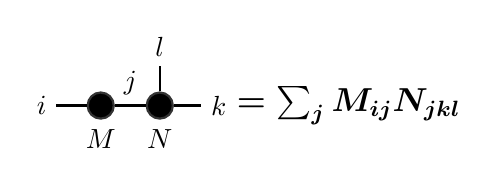
\begin{tikzpicture}
	\node[circle,draw=black!80,thick,fill=black,label=below:$M$] (M) at (0.75,0) {};
	\node[circle,draw=black!80,thick,fill=black,label=below:$N$] (N) at (1.5,0) {};
	\node (i) at (0,0) {$i$};
	\node (l) at (1.5,0.75) {$l$};
	\node (k) at (2.25,0) {$k$};
	\draw[thick, draw=black,label=above:] (M) -- node [above] {$j$} (N) {};
	\draw[thick, draw=black] (i) -- (M) {};
	\draw[thick, draw=black] (N) -- (k) {};
	\draw[thick, draw=black] (N) -- (l) {};
	\node at (3.9,0) {\large {\boldmath$= \sum_j M_{ij}N_{jkl}$}};
\end{tikzpicture}

		\caption{An example in tensor diagram notation}
	\end{mdframed}
\end{figure}

in \href{http://tensornetwork.org/diagrams/}{Tensor Diagram Notation} \\

Using this notation we can express Figure \ref{stencil timestep} in terms of tensors

\begin{figure}[H]
	\begin{mdframed}[backgroundcolor=myFigureColour]
		\newcommand{\graphLineSpacing}{0.5}
\newcommand{\graphTensorSpacing}{1}
\newcommand{\graphTensorTwoStart}{1.5*\graphTensorSpacing}
\newcommand{\graphTensorThreeStart}{\graphTensorTwoStart+ 2*\graphTensorSpacing}
\newcommand{\graphTensorFourStart}{\graphTensorThreeStart+ 2*\graphTensorSpacing}

\begin{tikzpicture}
	\node[circle,draw=black!80,thick,fill=black,label=left:$A_{t+1}$] (ATT) at (0,0) {};
	\node[circle,draw=black!80,thick,fill=black,label=left:${=}A_{t}$] (AT) at (\graphTensorTwoStart,0) {};
	\node[circle,draw=black!80,thick,fill=myGreen,label=above right:$X$] (X) at (\graphTensorTwoStart + \graphLineSpacing,\graphLineSpacing) {};
	\node[circle,draw=black!80,thick,fill=black,label=left:$+A_{t}$] (A) at (\graphTensorThreeStart,0) {};
	\node[circle,draw=black!80,thick,fill=myOrange,label=above right:$Y$] (Y) at (\graphTensorThreeStart + \graphLineSpacing,-\graphLineSpacing) {};

	\draw[thick, draw=black] (ATT) -- (0,\graphLineSpacing) -- (\graphLineSpacing,\graphLineSpacing) {};
	\draw[thick, draw=black] (ATT) -- (0,-\graphLineSpacing) -- (\graphLineSpacing,-\graphLineSpacing) {};

	\draw[thick, draw=black] (AT) -- (\graphTensorTwoStart,\graphLineSpacing) -- (X) -- (\graphTensorTwoStart + 2*\graphLineSpacing,\graphLineSpacing) {};
	\draw[thick, draw=black] (AT) -- (\graphTensorTwoStart,-\graphLineSpacing) -- (\graphTensorTwoStart + \graphLineSpacing, -\graphLineSpacing) {};

	\draw[thick, draw=black] (A) -- (\graphTensorThreeStart,\graphLineSpacing) -- (\graphTensorThreeStart + \graphLineSpacing,\graphLineSpacing) {};
	\draw[thick, draw=black] (A) -- (\graphTensorThreeStart,-\graphLineSpacing) -- (Y) -- (\graphTensorThreeStart + 2*\graphLineSpacing,-\graphLineSpacing) {};
\end{tikzpicture}
		\caption{A 2D stencil timestep update in tensor form}
		\label{tensor timestep}
	\end{mdframed}
\end{figure}

By self substitution of Figure \ref{tensor timestep} one time we can show two time steps as

\begin{figure}[H]
	\begin{mdframed}[backgroundcolor=myFigureColour]
		\renewcommand{\graphTensorSpacing}{1.1}
\renewcommand{\graphTensorTwoStart}{1.5*\graphTensorSpacing}
\renewcommand{\graphTensorThreeStart}{\graphTensorTwoStart+ 2*\graphTensorSpacing}
\renewcommand{\graphTensorFourStart}{\graphTensorThreeStart+ 2*\graphTensorSpacing}

\begin{tikzpicture}
	\node[circle,draw=black!80,thick,fill=black,label=left:$A_{t+2}$] (ATWO) at (0,0) {};
	\node[circle,draw=black!80,thick,fill=black,label=left:${=} A_{t}$] (A) at (\graphTensorTwoStart,0) {};
	\node[circle,draw=black!80,thick,fill=myGreen,label=above right:$X$] (X) at (\graphTensorTwoStart + \graphLineSpacing,\graphLineSpacing) {};
	\node[circle,draw=black!80,thick,fill=myGreen,label=above right:$X$] (X2) at (\graphTensorTwoStart + 2*\graphLineSpacing,\graphLineSpacing) {};
	\node[circle,draw=black!80,thick,fill=black,label=left:$+2A_{t}$] (AT) at (\graphTensorThreeStart,0) {};
	\node[circle,draw=black!80,thick,fill=myGreen,label=above right:$X$] (X3) at (\graphTensorThreeStart + \graphLineSpacing,\graphLineSpacing) {};
	\node[circle,draw=black!80,thick,fill=myOrange,label=above right:$Y$] (Y) at (\graphTensorThreeStart + \graphLineSpacing,-\graphLineSpacing) {};
	\node[circle,draw=black!80,thick,fill=black,label=left:$+A_{t}$] (ATT) at (\graphTensorFourStart,0) {};
	\node[circle,draw=black!80,thick,fill=myOrange,label=above right:$Y$] (Y2) at (\graphTensorFourStart + \graphLineSpacing,-\graphLineSpacing) {};
	\node[circle,draw=black!80,thick,fill=myOrange,label=above right:$Y$] (Y3) at (\graphTensorFourStart + 2*\graphLineSpacing,-\graphLineSpacing) {};

	\draw[thick, draw=black] (ATWO) -- (0,\graphLineSpacing) -- (\graphLineSpacing,\graphLineSpacing) {};
	\draw[thick, draw=black] (ATWO) -- (0,-\graphLineSpacing) -- (\graphLineSpacing,-\graphLineSpacing) {};

	\draw[thick, draw=black] (A) -- (\graphTensorTwoStart,\graphLineSpacing) -- (X) -- (X2) -- (\graphTensorTwoStart + 3*\graphLineSpacing,\graphLineSpacing)  {};
	\draw[thick, draw=black] (A) -- (\graphTensorTwoStart,-\graphLineSpacing) -- (\graphTensorTwoStart + \graphLineSpacing, -\graphLineSpacing) {};

	\draw[thick, draw=black] (AT) -- (\graphTensorThreeStart,\graphLineSpacing) -- (X3) -- (\graphTensorThreeStart + 2*\graphLineSpacing,\graphLineSpacing) {};
	\draw[thick, draw=black] (AT) -- (\graphTensorThreeStart,-\graphLineSpacing) -- (Y) -- (\graphTensorThreeStart + 2*\graphLineSpacing,-\graphLineSpacing) {};

	\draw[thick, draw=black] (ATT) -- (\graphTensorFourStart,\graphLineSpacing)  -- (\graphTensorFourStart + \graphLineSpacing,\graphLineSpacing)  {};
	\draw[thick, draw=black] (ATT) -- (\graphTensorFourStart,-\graphLineSpacing) -- (Y2) -- (Y3) -- (\graphTensorFourStart + 3*\graphLineSpacing, -\graphLineSpacing) {};
\end{tikzpicture}
		\caption{A 2D stencil timestep updatde twice}
	\end{mdframed}
\end{figure}

If you repeat this indefinitely you end up with the generalized form.

\begin{figure}[H]
	\begin{mdframed}[backgroundcolor=myFigureColour]
		
\renewcommand{\graphTensorSpacing}{1.1}
\renewcommand{\graphTensorTwoStart}{2.25*\graphTensorSpacing}
\[
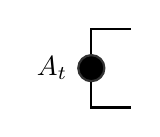
\begin{tikzpicture}[baseline=-0.65ex]
	\node[circle,draw=black!80,thick,fill=black,label=left:$A_{t}$] (ATT) at (0,0) {};

	\draw[thick, draw=black] (ATT) -- (0,\graphLineSpacing) -- (\graphLineSpacing,\graphLineSpacing) {};
	\draw[thick, draw=black] (ATT) -- (0,-\graphLineSpacing) -- (\graphLineSpacing,-\graphLineSpacing) {};
\end{tikzpicture}
=
\sum_{k=0}^{t}
{t \choose k}
\begin{tikzpicture}[baseline=-0.65ex]
	\node[circle,draw=black!80,thick,fill=black,label=left:$A_{0}$] (AT) at (\graphTensorTwoStart,0) {};
	\node[circle,draw=black!80,thick,fill=myGreen,label=above right:$X$] (X) at (\graphTensorTwoStart + 2*\graphLineSpacing,\graphLineSpacing) {};
	\node[circle,draw=black!80,thick,fill=myOrange,label=above right:$Y$] (Y) at (\graphTensorTwoStart + 2*\graphLineSpacing,-\graphLineSpacing) {};
	\node (k) at (\graphTensorTwoStart + 4*\graphLineSpacing,\graphLineSpacing) {$k$};
	\node (tk) at (\graphTensorTwoStart + 4*\graphLineSpacing,-\graphLineSpacing) {$t-k$};
	\node[circle,draw=black!80,thick,fill=myGreen,label=above right:$X$] (X1) at (\graphTensorTwoStart + 6*\graphLineSpacing,\graphLineSpacing) {};
	\node[circle,draw=black!80,thick,fill=myOrange,label=above right:$Y$] (Y1) at (\graphTensorTwoStart + 6*\graphLineSpacing,-\graphLineSpacing) {};

	\draw[thick, draw=black] (AT) -- (\graphTensorTwoStart,\graphLineSpacing) -- (\graphTensorTwoStart + \graphLineSpacing,\graphLineSpacing) ;
	\draw[thick, dotted] (\graphTensorTwoStart + \graphLineSpacing,\graphLineSpacing) -- (X) -- (k) -- (X1) -- (\graphTensorTwoStart + 7*\graphLineSpacing,\graphLineSpacing) {};
	\draw[thick, draw=black] (\graphTensorTwoStart + 7*\graphLineSpacing,\graphLineSpacing) -- (\graphTensorTwoStart + 8*\graphLineSpacing,\graphLineSpacing) {};

	\draw[thick, draw=black] (AT) -- (\graphTensorTwoStart,-\graphLineSpacing) -- (\graphTensorTwoStart + \graphLineSpacing,-\graphLineSpacing) {};
	\draw[thick, dotted] (\graphTensorTwoStart + \graphLineSpacing,-\graphLineSpacing) -- (Y) -- (tk) -- (Y1) -- (\graphTensorTwoStart + 7*\graphLineSpacing,-\graphLineSpacing) {};
	\draw[thick, draw=black] (\graphTensorTwoStart + 7*\graphLineSpacing,-\graphLineSpacing) -- (\graphTensorTwoStart + 8*\graphLineSpacing,-\graphLineSpacing) {};
\end{tikzpicture}
\]
		\caption{A 2D stencil timestep updated t times}
		\label{tensor timestep 2D}
	\end{mdframed}
\end{figure}

This can be generalized to 3D and ND in Fig \ref{tensor timestep 3D} and Fig \ref{tensor timestep ND} respectively.


\begin{figure}[H]
	\begin{mdframed}[backgroundcolor=myFigureColour]
		\renewcommand{\graphTensorSpacing}{1.1}
\renewcommand{\graphTensorTwoStart}{2.25*\graphTensorSpacing}
\[
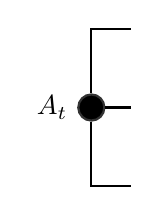
\begin{tikzpicture}[baseline=-0.65ex]
	\node[circle,draw=black!80,thick,fill=black,label=left:$A_{t}$] (ATT) at (0,0) {};

	\draw[thick, draw=black] (ATT) -- (0,2*\graphLineSpacing) -- (\graphLineSpacing,2*\graphLineSpacing) {};
	\draw[thick, draw=black] (ATT) -- (\graphLineSpacing,0) {};
	\draw[thick, draw=black] (ATT) -- (0,-2*\graphLineSpacing) -- (\graphLineSpacing,-2*\graphLineSpacing) {};
\end{tikzpicture}
=
\sum_{\substack{i,j,k\\ i+j+k=t}}
{t \choose {i,j,k}}
\begin{tikzpicture}[baseline=-0.65ex]
	\node[circle,draw=black!80,thick,fill=black,label=left:$A_{0}$] (AT) at (\graphTensorTwoStart,0) {};
	\node[circle,draw=black!80,thick,fill=myGreen,label=above right:$X$] (X) at (\graphTensorTwoStart + 2*\graphLineSpacing,2*\graphLineSpacing) {};
	\node[circle,draw=black!80,thick,fill=myGreen,label=above right:$X$] (X1) at (\graphTensorTwoStart + 6*\graphLineSpacing,2*\graphLineSpacing) {};
	\node[circle,draw=black!80,thick,fill=myOrange,label=above right:$Y$] (Y) at (\graphTensorTwoStart + 2*\graphLineSpacing,0) {};
	\node[circle,draw=black!80,thick,fill=myOrange,label=above right:$Y$] (Y1) at (\graphTensorTwoStart + 6*\graphLineSpacing,0) {};
	\node[circle,draw=black!80,thick,fill=myBlue,label=above right:$Z$] (Z) at (\graphTensorTwoStart + 2*\graphLineSpacing,-2*\graphLineSpacing) {};
	\node[circle,draw=black!80,thick,fill=myBlue,label=above right:$Z$] (Z1) at (\graphTensorTwoStart + 6*\graphLineSpacing,-2*\graphLineSpacing) {};

	\node (i) at (\graphTensorTwoStart + 4*\graphLineSpacing,2*\graphLineSpacing) {$i$};
	\node (j) at (\graphTensorTwoStart + 4*\graphLineSpacing,0) {$j$};
	\node (k) at (\graphTensorTwoStart + 4*\graphLineSpacing,-2*\graphLineSpacing) {$k$};
	
	\draw[thick, draw=black] (AT) -- (\graphTensorTwoStart,2*\graphLineSpacing) -- (\graphTensorTwoStart + \graphLineSpacing,2*\graphLineSpacing) ;
	\draw[thick, dotted] (\graphTensorTwoStart + \graphLineSpacing,2*\graphLineSpacing) -- (X) -- (i) -- (X1) -- (\graphTensorTwoStart + 7*\graphLineSpacing,2*\graphLineSpacing) {};
	\draw[thick, draw=black] (\graphTensorTwoStart + 7*\graphLineSpacing,2*\graphLineSpacing) -- (\graphTensorTwoStart + 8*\graphLineSpacing,2*\graphLineSpacing) {};

	\draw[thick, draw=black] (AT) -- (\graphTensorTwoStart + \graphLineSpacing,0) {};
	\draw[thick, dotted] (\graphTensorTwoStart + \graphLineSpacing,0) -- (Y) -- (j) -- (Y1) -- (\graphTensorTwoStart + 7*\graphLineSpacing,0) {};
	\draw[thick, draw=black] (\graphTensorTwoStart + 7*\graphLineSpacing,0) -- (\graphTensorTwoStart + 8*\graphLineSpacing,0) {};

	\draw[thick, draw=black] (AT) -- (\graphTensorTwoStart,-2*\graphLineSpacing) -- (\graphTensorTwoStart + \graphLineSpacing,-2*\graphLineSpacing) {};
	\draw[thick, dotted] (\graphTensorTwoStart + \graphLineSpacing,-2*\graphLineSpacing) -- (Z) -- (k) -- (Z1) -- (\graphTensorTwoStart + 7*\graphLineSpacing,-2*\graphLineSpacing) {};
	\draw[thick, draw=black] (\graphTensorTwoStart + 7*\graphLineSpacing,-2*\graphLineSpacing) -- (\graphTensorTwoStart + 8*\graphLineSpacing,-2*\graphLineSpacing) {};
\end{tikzpicture}
\]
		\caption{A 3D stencil timestep updated t times}
		\label{tensor timestep 3D}
	\end{mdframed}
\end{figure}

\begin{figure}[H]
	\begin{mdframed}[backgroundcolor=myFigureColour]
		\renewcommand{\graphTensorSpacing}{1}
\renewcommand{\graphTensorTwoStart}{2.25*\graphTensorSpacing}
\[
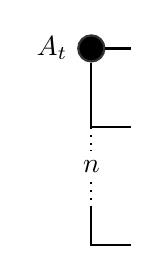
\begin{tikzpicture}[baseline=-7ex]
	\node[circle,draw=black!80,thick,fill=black,label=left:$A_{t}$] (ATT) at (0,0) {};
	\node (n) at (0,-3*\graphLineSpacing){$n$};

	\draw[thick, draw=black] (ATT) -- (\graphLineSpacing,0) {};
	\draw[thick, draw=black] (ATT) -- (0,-2*\graphLineSpacing) -- (\graphLineSpacing,-2*\graphLineSpacing) {};
	\draw[thick, dotted] (0,-2*\graphLineSpacing)  -- (n) -- (0,-4*\graphLineSpacing){};
	\draw[thick, draw=black] (0,-4*\graphLineSpacing) -- (0,-5*\graphLineSpacing) -- (\graphLineSpacing,-5*\graphLineSpacing) {};
\end{tikzpicture}
=
\sum_{\substack{i_1,i_2,\cdots,i_n\\ \sum_{k=0}^{n}{i_k} =t}}
{t \choose {i_1,i_2,\cdots,i_n}}
\begin{tikzpicture}[baseline=-7ex]s
	\node[circle,draw=black!80,thick,fill=black,label=left:$A_{0}$] (AT) at (\graphTensorTwoStart,0) {};
	\node[circle,draw=black!80,thick,fill=myBrown,label=above right:$X_1$] (X10) at (\graphTensorTwoStart + 2*\graphLineSpacing,0) {};
	\node[circle,draw=black!80,thick,fill=myBrown,label=above right:$X_1$] (X11) at (\graphTensorTwoStart + 6*\graphLineSpacing,0) {};
	\node[circle,draw=black!80,thick,fill=myBrown,label=above right:$X_2$] (X20) at (\graphTensorTwoStart + 2*\graphLineSpacing,-2*\graphLineSpacing) {};
	\node[circle,draw=black!80,thick,fill=myBrown,label=above right:$X_2$] (X21) at (\graphTensorTwoStart + 6*\graphLineSpacing,-2*\graphLineSpacing) {};
	\node[circle,draw=black!80,thick,fill=myBrown,label=above right:$X_N$] (XN0) at (\graphTensorTwoStart + 2*\graphLineSpacing,-5*\graphLineSpacing) {};
	\node[circle,draw=black!80,thick,fill=myBrown,label=above right:$X_N$] (XN1) at (\graphTensorTwoStart + 6*\graphLineSpacing,-5*\graphLineSpacing) {};

	\node (n) at (\graphTensorTwoStart,-3*\graphLineSpacing){$n$};

	\node (i1) at (\graphTensorTwoStart + 4*\graphLineSpacing,0) {$i_1$};
	\node (i2) at (\graphTensorTwoStart + 4*\graphLineSpacing,-2*\graphLineSpacing) {$i_2$};
	\node (in) at (\graphTensorTwoStart + 4*\graphLineSpacing,-5*\graphLineSpacing) {$i_n$};

	\draw[thick, draw=black] (AT) -- (\graphTensorTwoStart + \graphLineSpacing,0) {};
	\draw[thick, dotted] (\graphTensorTwoStart + \graphLineSpacing,0) -- (X10) -- (i1) -- (X11) -- (\graphTensorTwoStart + 7*\graphLineSpacing,0) {};
	\draw[thick, draw=black] (\graphTensorTwoStart + 7*\graphLineSpacing,0) -- (\graphTensorTwoStart + 8*\graphLineSpacing,0) {};

	\draw[thick, draw=black] (AT) -- (\graphTensorTwoStart,-2*\graphLineSpacing) -- (\graphTensorTwoStart + \graphLineSpacing,-2*\graphLineSpacing) {};
	\draw[thick, dotted] (\graphTensorTwoStart + \graphLineSpacing,-2*\graphLineSpacing) -- (X20) -- (i2) -- (X21) -- (\graphTensorTwoStart + 7*\graphLineSpacing,-2*\graphLineSpacing) {};
	\draw[thick, draw=black] (\graphTensorTwoStart + 7*\graphLineSpacing,-2*\graphLineSpacing) -- (\graphTensorTwoStart + 8*\graphLineSpacing,-2*\graphLineSpacing) {};

	\draw[thick, dotted] (\graphTensorTwoStart,-2*\graphLineSpacing)  -- (n) -- (\graphTensorTwoStart,-4*\graphLineSpacing){};
	\draw[thick, draw=black] (\graphTensorTwoStart,-4*\graphLineSpacing) -- (\graphTensorTwoStart,-5*\graphLineSpacing) -- (\graphTensorTwoStart + \graphLineSpacing,-5*\graphLineSpacing) {};
	\draw[thick, dotted] (\graphTensorTwoStart + \graphLineSpacing,-5*\graphLineSpacing) -- (XN0) -- (in) -- (XN1) -- (\graphTensorTwoStart + 7*\graphLineSpacing,-5*\graphLineSpacing) {};
	\draw[thick, draw=black] (\graphTensorTwoStart + 7*\graphLineSpacing,-5*\graphLineSpacing) -- (\graphTensorTwoStart + 8*\graphLineSpacing,-5*\graphLineSpacing) {};
\end{tikzpicture}
\]
		\caption{A ND stencil timestep updated t times}
		\label{tensor timestep ND}
	\end{mdframed}
\end{figure}

\subsection{eigendecomposition of toeplitz matrices}

Before moving onto simplifications we can make to the tensor expression we have in Fig \ref{tensor timestep 2D} - \ref{tensor timestep ND} we must look into how we can eigendecompose the transformation matrices we apply to each dimension.

\begin{figure}[H]
	\begin{mdframed}[backgroundcolor=myFigureColour]
		\renewcommand{\gridCellWidth}{0.3}
\renewcommand{\gridSize}{7}
\renewcommand{\gridSpacing}{0.9}
\renewcommand{\gridWidth}{\gridSize*\gridCellWidth}
\renewcommand{\gridAxisHorizontalCellColour}{myGreen}
\renewcommand{\gridAxisVerticalCellColour}{myOrange}
\renewcommand{\gridAxisMiddleColour}{myYellow}
\renewcommand{\gridTwoStart}{\gridSpacing}
\renewcommand{\gridThreeStart}{\gridTwoStart + \gridWidth + \gridSpacing}



\begin{tikzpicture}[every node/.style={minimum size=\gridCellWidth cm-\pgflinewidth, outer sep=0pt}]

%Grid 1

\node at (\gridSpacing/2,3.5*\gridCellWidth) {\large $X =$};

%Grid 2

\draw[step=\gridCellWidth cm,color=black] (\gridTwoStart,0) grid (\gridWidth + \gridTwoStart,\gridWidth);



\node[fill={\gridAxisHorizontalCellColour}] at (\gridTwoStart + 0.5*\gridCellWidth,5.5*\gridCellWidth) {};
\node[fill={\gridAxisHorizontalCellColour}] at (\gridTwoStart + 1.5*\gridCellWidth,4.5*\gridCellWidth) {};
\node[fill={\gridAxisHorizontalCellColour}] at (\gridTwoStart + 2.5*\gridCellWidth,3.5*\gridCellWidth) {};
\node[fill={\gridAxisHorizontalCellColour}] at (\gridTwoStart + 3.5*\gridCellWidth,2.5*\gridCellWidth) {};
\node[fill={\gridAxisHorizontalCellColour}] at (\gridTwoStart + 4.5*\gridCellWidth,1.5*\gridCellWidth) {};
\node[fill={\gridAxisHorizontalCellColour}] at (\gridTwoStart + 5.5*\gridCellWidth,0.5*\gridCellWidth) {};

\node at (\gridTwoStart + 0.5*\gridCellWidth,5.5*\gridCellWidth) {\footnotesize x1};
\node at (\gridTwoStart + 1.5*\gridCellWidth,4.5*\gridCellWidth) {\footnotesize x1};
\node at (\gridTwoStart + 2.5*\gridCellWidth,3.5*\gridCellWidth) {\footnotesize x1};
\node at (\gridTwoStart + 3.5*\gridCellWidth,2.5*\gridCellWidth) {\footnotesize x1};
\node at (\gridTwoStart + 4.5*\gridCellWidth,1.5*\gridCellWidth) {\footnotesize x1};
\node at (\gridTwoStart + 5.5*\gridCellWidth,0.5*\gridCellWidth) {\footnotesize x1};


\node[fill={\gridAxisMiddleColour}] at (\gridTwoStart + 0.5*\gridCellWidth,6.5*\gridCellWidth){};
\node[fill={\gridAxisMiddleColour}] at (\gridTwoStart + 1.5*\gridCellWidth,5.5*\gridCellWidth){};
\node[fill={\gridAxisMiddleColour}] at (\gridTwoStart + 2.5*\gridCellWidth,4.5*\gridCellWidth){};
\node[fill={\gridAxisMiddleColour}] at (\gridTwoStart + 3.5*\gridCellWidth,3.5*\gridCellWidth){};
\node[fill={\gridAxisMiddleColour}] at (\gridTwoStart + 4.5*\gridCellWidth,2.5*\gridCellWidth){};
\node[fill={\gridAxisMiddleColour}] at (\gridTwoStart + 5.5*\gridCellWidth,1.5*\gridCellWidth){};
\node[fill={\gridAxisMiddleColour}] at (\gridTwoStart + 6.5*\gridCellWidth,0.5*\gridCellWidth){};

\node at (\gridTwoStart + 0.5*\gridCellWidth,6.5*\gridCellWidth) {\tiny{$\frac{\text{m}}{n}$} };
\node at (\gridTwoStart + 1.5*\gridCellWidth,5.5*\gridCellWidth) {\tiny{$\frac{\text{m}}{n}$} };
\node at (\gridTwoStart + 2.5*\gridCellWidth,4.5*\gridCellWidth) {\tiny{$\frac{\text{m}}{n}$} };
\node at (\gridTwoStart + 3.5*\gridCellWidth,3.5*\gridCellWidth) {\tiny{$\frac{\text{m}}{n}$} };
\node at (\gridTwoStart + 4.5*\gridCellWidth,2.5*\gridCellWidth) {\tiny{$\frac{\text{m}}{n}$} };
\node at (\gridTwoStart + 5.5*\gridCellWidth,1.5*\gridCellWidth) {\tiny{$\frac{\text{m}}{n}$} };
\node at (\gridTwoStart + 6.5*\gridCellWidth,0.5*\gridCellWidth) {\tiny{$\frac{\text{m}}{n}$} };


\node[fill={\gridAxisHorizontalCellColour}] at (\gridTwoStart + 1.5*\gridCellWidth,6.5*\gridCellWidth) {};
\node[fill={\gridAxisHorizontalCellColour}] at (\gridTwoStart + 2.5*\gridCellWidth,5.5*\gridCellWidth) {};
\node[fill={\gridAxisHorizontalCellColour}] at (\gridTwoStart + 3.5*\gridCellWidth,4.5*\gridCellWidth) {};
\node[fill={\gridAxisHorizontalCellColour}] at (\gridTwoStart + 4.5*\gridCellWidth,3.5*\gridCellWidth) {};
\node[fill={\gridAxisHorizontalCellColour}] at (\gridTwoStart + 5.5*\gridCellWidth,2.5*\gridCellWidth) {};
\node[fill={\gridAxisHorizontalCellColour}] at (\gridTwoStart + 6.5*\gridCellWidth,1.5*\gridCellWidth) {};

\node at (\gridTwoStart + 1.5*\gridCellWidth,6.5*\gridCellWidth) {\footnotesize x2};
\node at (\gridTwoStart + 2.5*\gridCellWidth,5.5*\gridCellWidth) {\footnotesize x2};
\node at (\gridTwoStart + 3.5*\gridCellWidth,4.5*\gridCellWidth) {\footnotesize x2};
\node at (\gridTwoStart + 4.5*\gridCellWidth,3.5*\gridCellWidth) {\footnotesize x2};
\node at (\gridTwoStart + 5.5*\gridCellWidth,2.5*\gridCellWidth) {\footnotesize x2};
\node at (\gridTwoStart + 6.5*\gridCellWidth,1.5*\gridCellWidth) {\footnotesize x2};


%Grid 3

\draw[step=\gridCellWidth cm,color=black] (\gridThreeStart,0) grid (\gridWidth + \gridThreeStart,\gridWidth);

\node[fill={myGrey}] at (\gridThreeStart + 1.5*\gridCellWidth,5.5*\gridCellWidth){};
\node[fill={myGrey}] at (\gridThreeStart + 0.5*\gridCellWidth,6.5*\gridCellWidth){};
\node[fill={myGrey}] at (\gridThreeStart + 2.5*\gridCellWidth,4.5*\gridCellWidth){};
\node[fill={myGrey}] at (\gridThreeStart + 3.5*\gridCellWidth,3.5*\gridCellWidth){};
\node[fill={myGrey}] at (\gridThreeStart + 4.5*\gridCellWidth,2.5*\gridCellWidth){};
\node[fill={myGrey}] at (\gridThreeStart + 5.5*\gridCellWidth,1.5*\gridCellWidth){};
\node[fill={myGrey}] at (\gridThreeStart + 6.5*\gridCellWidth,0.5*\gridCellWidth){};

\node at (\gridThreeStart + 0.5*\gridCellWidth,6.5*\gridCellWidth) {\tiny{$\lambda_1$} };
\node at (\gridThreeStart + 1.5*\gridCellWidth,5.5*\gridCellWidth) {\tiny{$\lambda_2$} };
\node at (\gridThreeStart + 2.5*\gridCellWidth,4.5*\gridCellWidth) {\tiny{$\lambda_3$} };
\node at (\gridThreeStart + 3.5*\gridCellWidth,3.5*\gridCellWidth) {\tiny{$\lambda_4$} };
\node at (\gridThreeStart + 4.5*\gridCellWidth,2.5*\gridCellWidth) {\tiny{$\lambda_5$} };
\node at (\gridThreeStart + 5.5*\gridCellWidth,1.5*\gridCellWidth) {\tiny{$\lambda_6$} };
\node at (\gridThreeStart + 6.5*\gridCellWidth,0.5*\gridCellWidth) {\tiny{$\lambda_7$} };


%in between
\node at (\gridTwoStart + \gridWidth + \gridSpacing/2 ,3.5*\gridCellWidth){$=Q\cdot$};
\node at (\gridThreeStart + \gridWidth + \gridSpacing/2 ,3.5*\gridCellWidth){$\cdot Q^{-1}$};
% transpose
\end{tikzpicture}
		\caption{A ND stencil timestep updated t times}
	\end{mdframed}
\end{figure}

You can eigendecompose a tridiagonal toeplitz analytically and higher orders can be done incrementally \cite{bogoya2022fast}
The eigendecomposition for tridiagonal toeplitz matrices that arise from 3 wide stencils is as follows.


\[ i,j = 1:n\]
\[ {Q_X}_{i,i} = \frac{m}{2} + 2\sqrt{x1 x2}\cos{\frac{i\pi}{n+1}}\]
\[ {\Lambda_X}_{i,j} = (\frac{x1}{x2})^{\frac{j}{2}}\sin{\frac{ij\pi}{n+1}} \]

This eigendecomposition can be represented in tensor graph notation.

\begin{figure}[H]
	\begin{mdframed}[backgroundcolor=myFigureColour]
	
\renewcommand{\graphTensorSpacing}{1.1}
\renewcommand{\graphTensorTwoStart}{2.25*\graphTensorSpacing}
\[
\begin{tikzpicture}[baseline=-0.65ex]
	\node[circle,draw=black!80,thick,fill=myGreen,label=above:$X$] (X) at (0,0) {};
	\draw[thick, draw=black] (-\graphLineSpacing,0) -- (X) -- (\graphLineSpacing,0) {};
\end{tikzpicture}
=
\begin{tikzpicture}[baseline=-0.65ex]
	\node[circle,draw=black!80,thick,fill=black,label=above:$Q_X$] (Q) at (0,0) {};
	\node[circle,draw=black!80,thick,fill=myGrey,label=above:$\Lambda_X$] (LAMBDA) at (\graphTensorSpacing,0) {};
	\draw[thick] (\graphTensorSpacing - 0.2,0 + 0.2) -- (\graphTensorSpacing + 0.2,0 - 0.2) {};
	\node[circle,draw=black!80,thick,fill=black,label=above:$Q_X^{-1}$] (Q1) at (2*\graphTensorSpacing,0) {};

	\draw[thick, draw=black] (-\graphLineSpacing,0) -- (Q) -- (LAMBDA) -- (Q1) -- (2*\graphTensorSpacing + \graphLineSpacing,0) {};

\end{tikzpicture}
\]
	\caption{A tensor eigendecomposition}
\end{mdframed}
\end{figure}

Sequential matrix transformations by the same matrix can be eigendecomposed simply

\begin{figure}[H]
	\begin{mdframed}[backgroundcolor=myFigureColour]
	
\renewcommand{\graphTensorSpacing}{1.1}
\renewcommand{\graphTensorTwoStart}{2.25*\graphTensorSpacing}
\[
\begin{tikzpicture}[baseline=-0.65ex]
	\node[circle,draw=black!80,thick,fill=myGreen,label=above:$X$] (X) at (0,0) {};
	\node (i) at (\graphLineSpacing,0) {$i$};
	\node[circle,draw=black!80,thick,fill=myGreen,label=above:$X$] (X1) at (2*\graphLineSpacing,0) {};

	\draw[thick, draw=black] (-\graphLineSpacing,0) -- (X) {};
	\draw[thick, dotted] (X) -- (i) -- (X1) {};
	\draw[thick, draw=black]  (X1) -- (3*\graphLineSpacing,0){};
\end{tikzpicture}
=
\begin{tikzpicture}[baseline=-0.65ex]
	\node[circle,draw=black!80,thick,fill=black,label=above:$Q_X$] (Q) at (0,0) {};
	
	\node[circle,draw=black!80,thick,fill=myGrey,label=above:$\lambda_X^i$] (LAMBDA) at (\graphTensorSpacing,0) {};
	\draw[thick] (\graphTensorSpacing - 0.2,0 + 0.2) -- (\graphTensorSpacing + 0.2,0 - 0.2) {};

	\node[circle,draw=black!80,thick,fill=black,label=above:$Q_X^{-1}$] (Q1) at (2*\graphTensorSpacing,0) {};

	\draw[thick, draw=black] (-\graphLineSpacing,0) -- (Q) -- (LAMBDA) -- (Q1) -- (2*\graphTensorSpacing + \graphLineSpacing,0) {};

\end{tikzpicture}
\]
	\caption{A tensor eigendecomposition to the power of i}
\end{mdframed}
\end{figure}

This is because sequential $Q_X$ and $Q_X^{-1}$ cancel out.

\subsection{Hadamard product}

Before going any further we need to introduce the Hadamard product operator.
On a given tensor it is just an element wise multiplication. \\

$\circ$ the Hadamard Product means ${(A \circ B)}_{ij} = (A)_{ij} (B)_{ij}$ \\

\renewcommand{\graphTensorSpacing}{1}

\[
\sum_{\substack{i_1,i_2,\cdots,i_n\\ \sum_{k=1}^{n}{i_k} =t}}
\left(
{t \choose {i_1,i_2,\cdots,i_n}}
\begin{tikzpicture}[baseline=-7ex]s
	\node[circle,draw=black!80,thick,fill=black,label=left:$A$] (AT) at (0,-2*\graphLineSpacing) {};
	\node[circle,draw=black!80,thick,fill=myGrey,label=above right:$(\Lambda_1)^{i_1}$] (X1) at (0 + 2*\graphLineSpacing,0) {};
	\draw[thick] (0 + 2*\graphLineSpacing - 0.2,0 + 0.2) -- (0 + 2*\graphLineSpacing + 0.2,0 - 0.2) {};
	\node[circle,draw=black!80,thick,fill=myGrey,label=above right:$(\Lambda_2)^{i_2}$] (X2) at (0 + 2*\graphLineSpacing,-2*\graphLineSpacing) {};
	\draw[thick] (0 + 2*\graphLineSpacing - 0.2,-2*\graphLineSpacing + 0.2) -- (0 + 2*\graphLineSpacing + 0.2,-2*\graphLineSpacing - 0.2) {};
	\node[circle,draw=black!80,thick,fill=myGrey,label=above right:$(\Lambda_n)^{i_n}$] (XN0) at (0 + 2*\graphLineSpacing,-5*\graphLineSpacing) {};
	\draw[thick] (0 + 2*\graphLineSpacing - 0.2,-5*\graphLineSpacing + 0.2) -- (0 + 2*\graphLineSpacing + 0.2,-5*\graphLineSpacing - 0.2) {};

	\node (n) at (0,-3.5*\graphLineSpacing){$n$};

	\draw[thick, draw=black] (AT) -- (0,0) -- (X1) -- (0 + 3*\graphLineSpacing,0) {};

	\draw[thick, draw=black] (AT) -- (X2) -- (0 + 3*\graphLineSpacing,-2*\graphLineSpacing) -- (0 + 3*\graphLineSpacing,-2*\graphLineSpacing) {};

	\draw[thick, draw=black] (AT) -- (0,-2.5*\graphLineSpacing) {}; 
	\draw[thick, dotted] (0,-2.5*\graphLineSpacing)  -- (n) -- (0,-4.5*\graphLineSpacing){};
	\draw[thick, draw=black] (0,-4.5*\graphLineSpacing) -- (0,-5*\graphLineSpacing) -- (0 + \graphLineSpacing,-5*\graphLineSpacing) -- (XN0)  -- (0 + 3*\graphLineSpacing,-5*\graphLineSpacing) {};
\end{tikzpicture}
\right)
\equiv
A
\circ
\left(
\sum_{k=1}^n
\begin{tikzpicture}[baseline=-7ex]s
	\node[circle,draw=black!80,thick,fill=black,label=left:$I$] (I) at (0,-2*\graphLineSpacing) {};
	\node[circle,draw=black!80,thick,fill=myGrey,label=above right:$\Lambda_{k}$] (X2) at (0 + 2*\graphLineSpacing,-2*\graphLineSpacing) {};
	\draw[thick] (0 + 2*\graphLineSpacing - 0.2,-2*\graphLineSpacing + 0.2) -- (0 + 2*\graphLineSpacing + 0.2,-2*\graphLineSpacing - 0.2) {};

	\node (n) at (0,-3.5*\graphLineSpacing){$n$};

	\draw[thick, draw=black] (AT) -- (0,0) --  (0 + 2*\graphLineSpacing,0) {};

	\draw[thick, draw=black, label=above:] (AT) -- node [above] {$k$} (X2) -- (0 + 3*\graphLineSpacing,-2*\graphLineSpacing) -- (0 + 3*\graphLineSpacing,-2*\graphLineSpacing) {};

	\draw[thick, draw=black] (AT) -- (0,-2.5*\graphLineSpacing) {}; 
	\draw[thick, dotted] (0,-2.5*\graphLineSpacing)  -- (n) -- (0,-4.5*\graphLineSpacing){};
	\draw[thick, draw=black] (0,-4.5*\graphLineSpacing) -- (0,-5*\graphLineSpacing) -- (0 + \graphLineSpacing,-5*\graphLineSpacing) -- (0 + 2*\graphLineSpacing,-5*\graphLineSpacing) {};
\end{tikzpicture}
\right)^{\circ t}
\] \\
\[ A
\circ
\left(
\sum_{k=1}^n
	\begin{tikzpicture}[baseline=-7ex]s
	\node[circle,draw=black!80,thick,fill=black,label=left:$I$] (I) at (0,-2*\graphLineSpacing) {};
	\node[circle,draw=black!80,thick,fill=myGrey,label=above right:$\Lambda_{k}$] (X2) at (0 + 2*\graphLineSpacing,-2*\graphLineSpacing) {};
	\draw[thick] (0 + 2*\graphLineSpacing - 0.2,-2*\graphLineSpacing + 0.2) -- (0 + 2*\graphLineSpacing + 0.2,-2*\graphLineSpacing - 0.2) {};

	\node (n) at (0,-3.5*\graphLineSpacing){$n$};

	\draw[thick, draw=black] (AT) -- (0,0) --  (0 + 2*\graphLineSpacing,0) {};

	\draw[thick, draw=black, label=above:] (AT) -- node [above] {$k$} (X2) -- (0 + 3*\graphLineSpacing,-2*\graphLineSpacing) -- (0 + 3*\graphLineSpacing,-2*\graphLineSpacing) {};

	\draw[thick, draw=black] (AT) -- (0,-2.5*\graphLineSpacing) {}; 
	\draw[thick, dotted] (0,-2.5*\graphLineSpacing)  -- (n) -- (0,-4.5*\graphLineSpacing){};
	\draw[thick, draw=black] (0,-4.5*\graphLineSpacing) -- (0,-5*\graphLineSpacing) -- (0 + \graphLineSpacing,-5*\graphLineSpacing) -- (0 + 2*\graphLineSpacing,-5*\graphLineSpacing) {};
\end{tikzpicture} \right)^{\circ t}_{i_1, i_2, \cdots, i_n}
\equiv A_{i_1, i_2, \cdots, i_n} \left( \sum_{k=1}^{n} {(\Lambda_k)}_{i_k,i_k} \right)^t\]



\subsection{3D Formula}
\renewcommand{\graphTensorSpacing}{1.75}

\[ A_t = 
\left(
\left(
\begin{tikzpicture}[baseline=-7ex]s
	\node[circle,draw=black!80,thick,fill=black,label=left:$A_{0}$] (AT) at (0,-2*\graphLineSpacing) {};
	\node[circle,draw=black!80,thick,fill=myGreen,label=above right:$Q_{X}$] (X10) at (0 + 2*\graphLineSpacing,0) {};
	\node[circle,draw=black!80,thick,fill=myOrange,label=above right:$Q_{Y}$] (X20) at (0 + 2*\graphLineSpacing,-2*\graphLineSpacing) {};
	\node[circle,draw=black!80,thick,fill=myBlue,label=above right:$Q_{Z}$] (XN0) at (0 + 2*\graphLineSpacing,-4*\graphLineSpacing) {};

	\draw[thick, draw=black] (AT) -- (0,0) -- (0 + \graphLineSpacing,0) -- (X10) -- (0 + 3*\graphLineSpacing,0) {};

	\draw[thick, draw=black] (AT) -- (0 + \graphLineSpacing,-2*\graphLineSpacing) -- (X20) -- (0 + 3*\graphLineSpacing,-2*\graphLineSpacing){};

	\draw[thick, draw=black] (AT) -- (0,-4*\graphLineSpacing) -- (XN0) -- (0 + 3*\graphLineSpacing,-4*\graphLineSpacing) {};
\end{tikzpicture}
\right)
\circ
\left(
\begin{tikzpicture}[baseline=-7ex]s
	\node[circle,draw=black!80,thick,fill=black,label=left:$I$] (I1) at (0,-2*\graphLineSpacing) {};
	\node[circle,draw=black!80,thick,fill=myGrey,label=above right:$\Lambda_{X}$] (X1) at (0 + 1*\graphLineSpacing,0) {};
	\draw[thick] (0 + 1*\graphLineSpacing - 0.2,0 + 0.2) -- (0 + 1*\graphLineSpacing + 0.2,0 - 0.2) {};

	\draw[thick, draw=black] (I1) -- (0,0) --  (X1) -- (0 + 2*\graphLineSpacing,0) {};
	\draw[thick, draw=black, label=above:] (I1)  -- (0 + 1*\graphLineSpacing,-2*\graphLineSpacing) {};
	\draw[thick, draw=black] (I1) --  (0,-4*\graphLineSpacing) -- (0 + 1*\graphLineSpacing,-4*\graphLineSpacing) {};

	\node[circle,draw=black!80,thick,fill=black,label=left:$I$] (I2) at (\graphTensorSpacing,-2*\graphLineSpacing) {};
	\node[circle,draw=black!80,thick,fill=myGrey,label=above right:$\Lambda_{Y}$] (X2) at (\graphTensorSpacing + 1*\graphLineSpacing,-2*\graphLineSpacing) {};
	\draw[thick] (\graphTensorSpacing + 1*\graphLineSpacing - 0.2,-2*\graphLineSpacing + 0.2) -- (\graphTensorSpacing + 1*\graphLineSpacing + 0.2,-2*\graphLineSpacing - 0.2) {};

	\draw[thick, draw=black] (I2) -- (\graphTensorSpacing,0) --  (\graphTensorSpacing + 1*\graphLineSpacing,0) {};
	\draw[thick, draw=black, label=above:] (I2) -- (X2) -- (\graphTensorSpacing + 2*\graphLineSpacing,-2*\graphLineSpacing) {};
	\draw[thick, draw=black] (I2) --  (\graphTensorSpacing,-4*\graphLineSpacing) -- (\graphTensorSpacing + 1*\graphLineSpacing,-4*\graphLineSpacing) {};

	\node[circle,draw=black!80,thick,fill=black,label=left:$I$] (I3) at (2.25*\graphTensorSpacing,-2*\graphLineSpacing) {};
	\node[circle,draw=black!80,thick,fill=myGrey,label=above right:$\Lambda_{Z}$] (X3) at (2.25*\graphTensorSpacing + 1*\graphLineSpacing,-4*\graphLineSpacing) {};
	\draw[thick] (2.25*\graphTensorSpacing + 1*\graphLineSpacing - 0.2,-4*\graphLineSpacing + 0.2) -- (2.25*\graphTensorSpacing + 1*\graphLineSpacing + 0.2,-4*\graphLineSpacing - 0.2) {};

	\draw[thick, draw=black] (I3) -- (2.25*\graphTensorSpacing,0) --  (2.25*\graphTensorSpacing + 1*\graphLineSpacing,0) {};
	\draw[thick, draw=black, label=above:] (I3) --  (2.25*\graphTensorSpacing + 1*\graphLineSpacing,-2*\graphLineSpacing) {};
	\draw[thick, draw=black] (I3) --  (2.25*\graphTensorSpacing,-4*\graphLineSpacing) -- (X3) -- (2.25*\graphTensorSpacing + 2*\graphLineSpacing,-4*\graphLineSpacing) {};
	
	\node (plus1) at (1.85*\graphTensorSpacing,-2*\graphLineSpacing) {\large +};
	\node (plus2) at (0.6*\graphTensorSpacing,-2*\graphLineSpacing) {\large +};

\end{tikzpicture}
\right)^{\circ t}
\right)
\begin{tikzpicture}[baseline=-7ex]s
	\node[circle,draw=black!80,thick,fill=myGreen,label=above right:$Q^{-1}_{X}$] (X10) at (0 + 2*\graphLineSpacing,0) {};
	\node[circle,draw=black!80,thick,fill=myOrange,label=above right:$Q^{-1}_{Y}$] (X20) at (0 + 2*\graphLineSpacing,-2*\graphLineSpacing) {};
	\node[circle,draw=black!80,thick,fill=myBlue,label=above right:$Q^{-1}_{Z}$] (XN0) at (0 + 2*\graphLineSpacing,-4*\graphLineSpacing) {};

	\draw[thick, draw=black] (0,0) -- (X10) -- (0 + 3*\graphLineSpacing,0) {};

	\draw[thick, draw=black] (0,-2*\graphLineSpacing) -- (X20) -- (0 + 3*\graphLineSpacing,-2*\graphLineSpacing){};

	\draw[thick, draw=black] (0,-4*\graphLineSpacing) -- (XN0) -- (0 + 3*\graphLineSpacing,-4*\graphLineSpacing) {};
\end{tikzpicture}
\]
\renewcommand{\gridCellWidth}{0.5}
\renewcommand{\gridWidth}{\gridCellWidth*5}


\[
\left(
\begin{tikzpicture}[baseline=-7ex]s
	\node[circle,draw=black!80,thick,fill=black,label=left:$I$] (I1) at (0,-2*\graphLineSpacing) {};
	\node[circle,draw=black!80,thick,fill=myGrey,label=above right:$\Lambda_{X}$] (X1) at (0 + 1*\graphLineSpacing,0) {};
	\draw[thick] (0 + 1*\graphLineSpacing - 0.2,0 + 0.2) -- (0 + 1*\graphLineSpacing + 0.2,0 - 0.2) {};

	\draw[thick, draw=black] (I1) -- (0,0) --  (X1) -- (0 + 2*\graphLineSpacing,0) {};
	\draw[thick, draw=black, label=above:] (I1)  -- (0 + 1*\graphLineSpacing,-2*\graphLineSpacing) {};
	\draw[thick, draw=black] (I1) --  (0,-4*\graphLineSpacing) -- (0 + 1*\graphLineSpacing,-4*\graphLineSpacing) {};

	\node[circle,draw=black!80,thick,fill=black,label=left:$I$] (I2) at (\graphTensorSpacing,-2*\graphLineSpacing) {};
	\node[circle,draw=black!80,thick,fill=myGrey,label=above right:$\Lambda_{Y}$] (X2) at (\graphTensorSpacing + 1*\graphLineSpacing,-2*\graphLineSpacing) {};
	\draw[thick] (\graphTensorSpacing + 1*\graphLineSpacing - 0.2,-2*\graphLineSpacing + 0.2) -- (\graphTensorSpacing + 1*\graphLineSpacing + 0.2,-2*\graphLineSpacing - 0.2) {};

	\draw[thick, draw=black] (I2) -- (\graphTensorSpacing,0) --  (\graphTensorSpacing + 1*\graphLineSpacing,0) {};
	\draw[thick, draw=black, label=above:] (I2) -- (X2) -- (\graphTensorSpacing + 2*\graphLineSpacing,-2*\graphLineSpacing) {};
	\draw[thick, draw=black] (I2) --  (\graphTensorSpacing,-4*\graphLineSpacing) -- (\graphTensorSpacing + 1*\graphLineSpacing,-4*\graphLineSpacing) {};

	\node[circle,draw=black!80,thick,fill=black,label=left:$I$] (I3) at (2.25*\graphTensorSpacing,-2*\graphLineSpacing) {};
	\node[circle,draw=black!80,thick,fill=myGrey,label=above right:$\Lambda_{Z}$] (X3) at (2.25*\graphTensorSpacing + 1*\graphLineSpacing,-4*\graphLineSpacing) {};
	\draw[thick] (2.25*\graphTensorSpacing + 1*\graphLineSpacing - 0.2,-4*\graphLineSpacing + 0.2) -- (2.25*\graphTensorSpacing + 1*\graphLineSpacing + 0.2,-4*\graphLineSpacing - 0.2) {};

	\draw[thick, draw=black] (I3) -- (2.25*\graphTensorSpacing,0) --  (2.25*\graphTensorSpacing + 1*\graphLineSpacing,0) {};
	\draw[thick, draw=black, label=above:] (I3) --  (2.25*\graphTensorSpacing + 1*\graphLineSpacing,-2*\graphLineSpacing) {};
	\draw[thick, draw=black] (I3) --  (2.25*\graphTensorSpacing,-4*\graphLineSpacing) -- (X3) -- (2.25*\graphTensorSpacing + 2*\graphLineSpacing,-4*\graphLineSpacing) {};
	
	\node (plus1) at (1.85*\graphTensorSpacing,-2*\graphLineSpacing) {\large +};
	\node (plus2) at (0.6*\graphTensorSpacing,-2*\graphLineSpacing) {\large +};

\end{tikzpicture}
\right)^{\circ t}_{i,j,k}
= (({\Lambda_X})_{i,i} + ({\Lambda_Y}_{j,j}) + ({\Lambda_Z}_{k,k}))^t
\]


\subsection{Generalized Formula}
\[ A_t = 
\left(
\left(
\begin{tikzpicture}[baseline=-7ex]s
	\node[circle,draw=black!80,thick,fill=black,label=left:$A_{0}$] (AT) at (0,-2*\graphLineSpacing) {};
	\node[circle,draw=black!80,thick,fill=myBrown,label=above right:$Q_{X_1}$] (X10) at (0 + 2*\graphLineSpacing,0) {};
	\node[circle,draw=black!80,thick,fill=myBrown,label=above right:$Q_{X_2}$] (X20) at (0 + 2*\graphLineSpacing,-2*\graphLineSpacing) {};
	\node[circle,draw=black!80,thick,fill=myBrown,label=above right:$Q_{X_n}$] (XN0) at (0 + 2*\graphLineSpacing,-5*\graphLineSpacing) {};

	\node (n) at (0,-3.5*\graphLineSpacing){$n$};


	\draw[thick, draw=black] (AT) -- (0,0) -- (0 + \graphLineSpacing,0) -- (X10) -- (0 + 3*\graphLineSpacing,0) {};

	\draw[thick, draw=black] (AT) -- (0 + \graphLineSpacing,-2*\graphLineSpacing) -- (X20) -- (0 + 3*\graphLineSpacing,-2*\graphLineSpacing){};

	\draw[thick, draw=black] (AT) -- (0,-3*\graphLineSpacing);
	\draw[thick, dotted] (0,-3*\graphLineSpacing)  -- (n) -- (0,-4.5*\graphLineSpacing){};
	\draw[thick, draw=black] (0,-4.5*\graphLineSpacing) -- (0,-5*\graphLineSpacing) -- (0 + \graphLineSpacing,-5*\graphLineSpacing) -- (XN0) -- (0 + 3*\graphLineSpacing,-5*\graphLineSpacing) {};
\end{tikzpicture}
\right)
\circ
\left(
\sum_{k=1}^n
	\begin{tikzpicture}[baseline=-7ex]s
	\node[circle,draw=black!80,thick,fill=black,label=left:$I$] (I) at (0,-2*\graphLineSpacing) {};
	\node[circle,draw=black!80,thick,fill=myGrey,label=above right:$\Lambda_{X_k}$] (X2) at (0 + 2*\graphLineSpacing,-2*\graphLineSpacing) {};
	\draw[thick] (0 + 2*\graphLineSpacing - 0.2,-2*\graphLineSpacing + 0.2) -- (0 + 2*\graphLineSpacing + 0.2,-2*\graphLineSpacing - 0.2) {};

	\node (n) at (0,-3.5*\graphLineSpacing){$n$};

	\draw[thick, draw=black] (AT) -- (0,0) --  (0 + 2*\graphLineSpacing,0) {};

	\draw[thick, draw=black, label=above:] (AT) -- node [above] {$k$} (X2) -- (0 + 3*\graphLineSpacing,-2*\graphLineSpacing) -- (0 + 3*\graphLineSpacing,-2*\graphLineSpacing) {};

	\draw[thick, draw=black] (AT) -- (0,-2.5*\graphLineSpacing) {}; 
	\draw[thick, dotted] (0,-2.5*\graphLineSpacing)  -- (n) -- (0,-4.5*\graphLineSpacing){};
	\draw[thick, draw=black] (0,-4.5*\graphLineSpacing) -- (0,-5*\graphLineSpacing) -- (0 + \graphLineSpacing,-5*\graphLineSpacing) -- (0 + 2*\graphLineSpacing,-5*\graphLineSpacing) {};
\end{tikzpicture} 
\right)^{\circ t}
\right)
\begin{tikzpicture}[baseline=-7ex]s
	\node[circle,draw=black!80,thick,fill=myBrown,label=above right:$Q^{-1}_{X_1}$] (X10) at (0 + 2*\graphLineSpacing,0) {};
	\node[circle,draw=black!80,thick,fill=myBrown,label=above right:$Q^{-1}_{X_2}$] (X20) at (0 + 2*\graphLineSpacing,-2*\graphLineSpacing) {};
	\node[circle,draw=black!80,thick,fill=myBrown,label=above right:$Q^{-1}_{X_n}$] (XN0) at (0 + 2*\graphLineSpacing,-5*\graphLineSpacing) {};

	\draw[thick, draw=black] (0,0) -- (X10) -- (0 + 3*\graphLineSpacing,0) {};

	\draw[thick, draw=black] (0,-2*\graphLineSpacing) -- (X20) -- (0 + 3*\graphLineSpacing,-2*\graphLineSpacing){};

	\draw[thick, dotted] (0,-3.5*\graphLineSpacing) -- ( 3*\graphLineSpacing,-3.5*\graphLineSpacing) {};

	\draw[thick, draw=black] (0,-5*\graphLineSpacing) -- (XN0) -- (0 + 3*\graphLineSpacing,-5*\graphLineSpacing) {};
\end{tikzpicture}
\]

\begin{filecontents*}{data/data1.csv}
	Size,TensorStencil,Devito,Error
	50,0.005018,0.007894,0.000002
	100,0.02809,0.076949,0.000003
	150,0.101568,0.205237,0.000006
	200,0.237379,0.549409,0.000009
	250,0.477033,1.323531,0.000012
	300,0.845301,2.743135,0.000004
	350,1.40546,5.197527,0.000045
	400,2.103525,8.888937,0.000014
	450,3.000352,14.547453,0.000027
	500,4.309026,22.966639,0.000013
	550,5.708703,34.023224,0.000044
	600,7.549911,50.373158,0
	650,10.571026,73.569817,0.000031
	700,15.045691,108.983444,0.000016
	750,16.388805,133.701202,0.000034
	800,21.642071,177.168427,0.000028
	850,24.640459,235.159698,0.000029
	900,30.80517,297.78067,0.00003
	950,38.120262,377.148132,0.000028
	1000,44.858974,469.869049,0.000045
\end{filecontents*}

\begin{filecontents*}{data/data2.csv}
	Size,TensorStencil,Devito,Error
	50, 4.228271, 2.330200, 0.000001
	100, 4.392849, 4.588415, 0.000002
	150, 4.994750, 6.917814, 0.000003
	200, 4.188376, 9.386390, 0.000005
	250, 4.201744, 11.542141, 0.000006
	300, 4.927461, 13.890500, 0.000008
	350, 4.236063, 16.138432, 0.000009
	400, 4.302618, 18.459612, 0.000010
	450, 4.222175, 20.967630, 0.000012
	500, 4.307445, 23.298811, 0.000013
	550, 4.325422, 25.430765, 0.000014
	600, 4.216995, 28.123375, 0.000016
	650, 5.049333, 33.346359, 0.000017
	700, 4.539420, 33.367851, 0.000018
	750, 4.260931, 34.197765, 0.000020
	800, 4.310477, 37.090954, 0.000021
	850, 4.264150, 41.915268, 0.000023
	900, 4.312349, 41.698330, 0.000024
	950, 4.245051, 44.506187, 0.000025
\end{filecontents*}

\begin{figure}[H]
	\begin{mdframed}[backgroundcolor=myFigureColour]
	\begin{tikzpicture}
		\begin{axis} [ymode=log,ymax = 1000,xmax = 1050, ylabel={time},xlabel={size and iterations},legend pos=south east]
		\addplot table [x=Size,y=Devito, col sep=comma] {data/data1.csv};
		\addplot table [x=Size,y=TensorStencil, col sep=comma] {data/data1.csv};
		\addlegendentry{Devito}
		\addlegendentry{TensorStencil}
		\end{axis}
	\end{tikzpicture}
	\caption{Size and Iterations Graph}
	\end{mdframed}
\end{figure}
The percent error of the L2 norm of the final data of tensor stencil and the Devito result
\begin{figure}[H]
	\begin{mdframed}[backgroundcolor=myFigureColour]
	\begin{tikzpicture}
		\begin{axis} [ylabel={percent error},xlabel={size and iterations},legend pos=south east]
		\addplot table [x=Size,y=Error, col sep=comma] {data/data1.csv};
		\addlegendentry{L2 Norm}
		\end{axis}
	\end{tikzpicture}
	\caption{Error Graph}
	\end{mdframed}
\end{figure}
For a $500^3$ data set comparing increasing iterations for Devito and TensorStencil
\begin{figure}[H]
	\begin{mdframed}[backgroundcolor=myFigureColour]
	\begin{tikzpicture}
		\begin{axis} [ymode=log,ymax = 100,xmax = 1050, ylabel={time},xlabel={iterations},legend pos=south east]
		\addplot table [x=Size,y=Devito, col sep=comma] {data/data2.csv};
		\addplot table [x=Size,y=TensorStencil, col sep=comma] {data/data2.csv};
		\addlegendentry{Devito}
		\addlegendentry{TensorStencil}
		\end{axis}
	\end{tikzpicture}
	\caption{Iterations graph}
	\end{mdframed}
\end{figure}

% \section{Proof}

% Todo
% \section{Complexity}
% Todo
% \section{Results}
% Todo

\bibliographystyle{ieeetr}
\bibliography{citation}

\end{document}